\section{Extended Related Work}
\label{Appendix: Extended Related Work}
In this section, we provide an extended related work to supplement the related work presented in the main body.

\textbf{Sample-Efficient VRL.}~~
Prohibitive sample complexity has been identified as the primary obstacle hindering the real-world applications of VRL~\citep{SAC-AE}.
Previous studies ascribe this inefficiency to VRL's requirements to concurrently optimize task-specific policies and learn compact state representations from high-dimensional observations.
As a result, significant efforts have been directed towards improving sample efficiency through the training of a more potent \textit{encoder}.
The most representative approaches design \textit{auxiliary representation tasks} to complement the RL objective, including pixel or latent reconstruction~\citep{SAC-AE, MLR}, future prediction~\citep{PI-SAC, SPR, Playvirtual}, and contrastive learning for instance~\citep{CURL, CCLF, DRIBO} or temporal discrimination~\citep{M-CURL, CPC, CCFDM, DRIML}.
Another approach is to \textit{pre-train a visual encoder} that enables efficient adaptation to downstream tasks~\citep{RRL,MVP,PVR,R3M}.
However, recent empirical studies suggest that these methods do not consistently improve training efficiency~\citep{Does_SSL, Learning-from-Scratch, ma2023learning}, indicating that insufficient representation may not be the primary bottleneck hindering the sample efficiency of current algorithms.
Our findings in Section~\ref{Sec: Modules} provide a compelling explanation for the limited impact of enhanced representation: the plasticity loss within the critic module is the primary constraint on VRL's sample efficiency.

\textbf{Plasticity Loss in Continual Learning vs. in Reinforcement Learning.}~~
Continual Learning (CL) aims to continuously acquire new tasks, referred to as plasticity, without forgetting previously learned tasks, termed stability. A primary challenge in CL is managing the stability-plasticity trade-off. Although online reinforcement learning (RL) exhibits characteristics of plasticity due to its non-stationary learning targets, there are fundamental differences between CL and RL. 
Firstly, online RL typically begins its learning process from scratch, which can lead to limited training data in the early stages. This scarcity of data can subsequently result in a loss of plasticity early on. Secondly, RL usually doesn't require an agent to learn multiple policies. Therefore, any decline in plasticity during the later stages won't significantly impact its overall performance.

\textbf{Measurement Metrics of Plasticity.}~~
\label{Appendix: Measurement Metrics of Plasticity}
Several metrics are available to assess plasticity, including weight norm, feature rank, visualization of loss landscape, and the fraction of active units (FAU). The weight norm (commonly of both encoder and head) serves a dual purpose: it not only acts as a criterion to determine when to maintain plasticity but also offers a direct method to regulate plasticity through L2 regularization~\citep{dormant_neuron, Plasticity_Injection}. However, \citet{Plasticity_Injection} show that the weight norm is sensitive to environments and cannot address the plasticity by controlling itself. The feature rank can be also regarded as a proxy metric for plasticity loss~\citep{implicit_under-parameterization, capacity_loss}. Although the feature matrices used by these two works are slightly different, they correlate the feature rank with performance collapse. Nevertheless, \citet{gulcehre2022empirical} observe that the correlation appears in restricted settings. Furthermore, the loss landscape has been drawing increasing attention for its ability to directly reflect the gradients in backpropagation. Still, computing the network's Hessian concerning a loss function and the gradient covariance can be computationally demanding~\citep{understanding_plasticity}. Our proposed method aims to obtain a reliable criterion without too much additional computation cost, and leverage it to guide the plasticity maintenance. We thus settled on the widely-recognized and potent metric, FAU, for assessing plasticity~\citep{dormant_neuron, plasticity_loss_CRL}. This metric provides an upper limit on the count of inactive units. As shown in Figure~\ref{fig:arr_main_result}, the experimental results validate that A-RR based on FAU significantly outperforms static RR baselines. Although FAU's efficacy is evident in various studies, including ours, its limitations in convolutional networks are highlighted by~\citep{understanding_plasticity}. Therefore, we advocate for future work to introduce a comprehensive and resilient plasticity metric.

\newpage
\section{Extended Experiment Results}
\subsection{Reset}
\label{Appendix: Reset}
To enhance the plasticity of the agent's network, the \textit{Reset} method periodically re-initializes the parameters of its last few layers, while preserving the replay buffer. In Figure~\ref{appendix_fig:reset}, we present additional experiments on six DMC tasks, exploring four scenarios: with and without the inclusion of both Reset and DA. Although reset is widely acknowledged for its efficacy in counteracting the adverse impacts of plasticity loss, our findings suggest its effectiveness largely hinges on the hyper-parameters determining the reset interval, as depicted in Figure~\ref{appendix_fig:reset_interval}.
\begin{figure}[ht]
  \centering
  \vspace{-\baselineskip}
  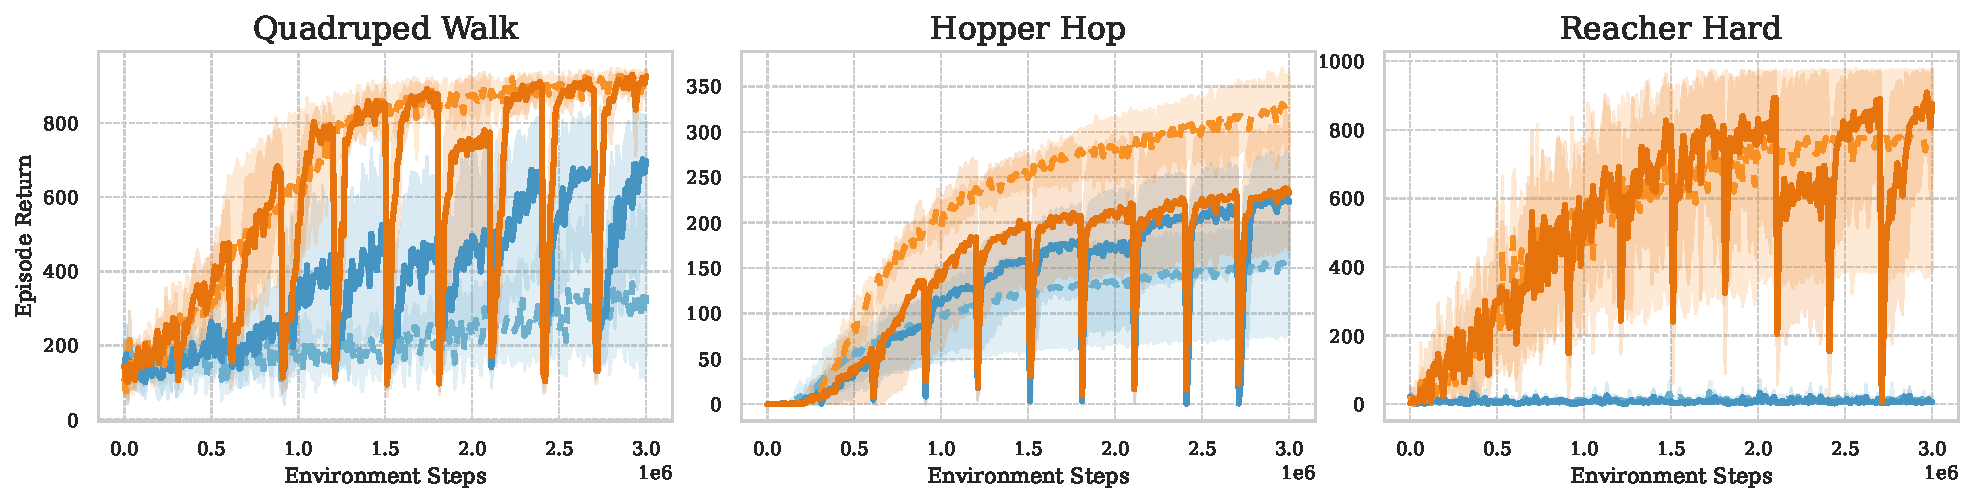
\includegraphics[width=\textwidth]{Figures/5Appendix/reset_DA.pdf}
  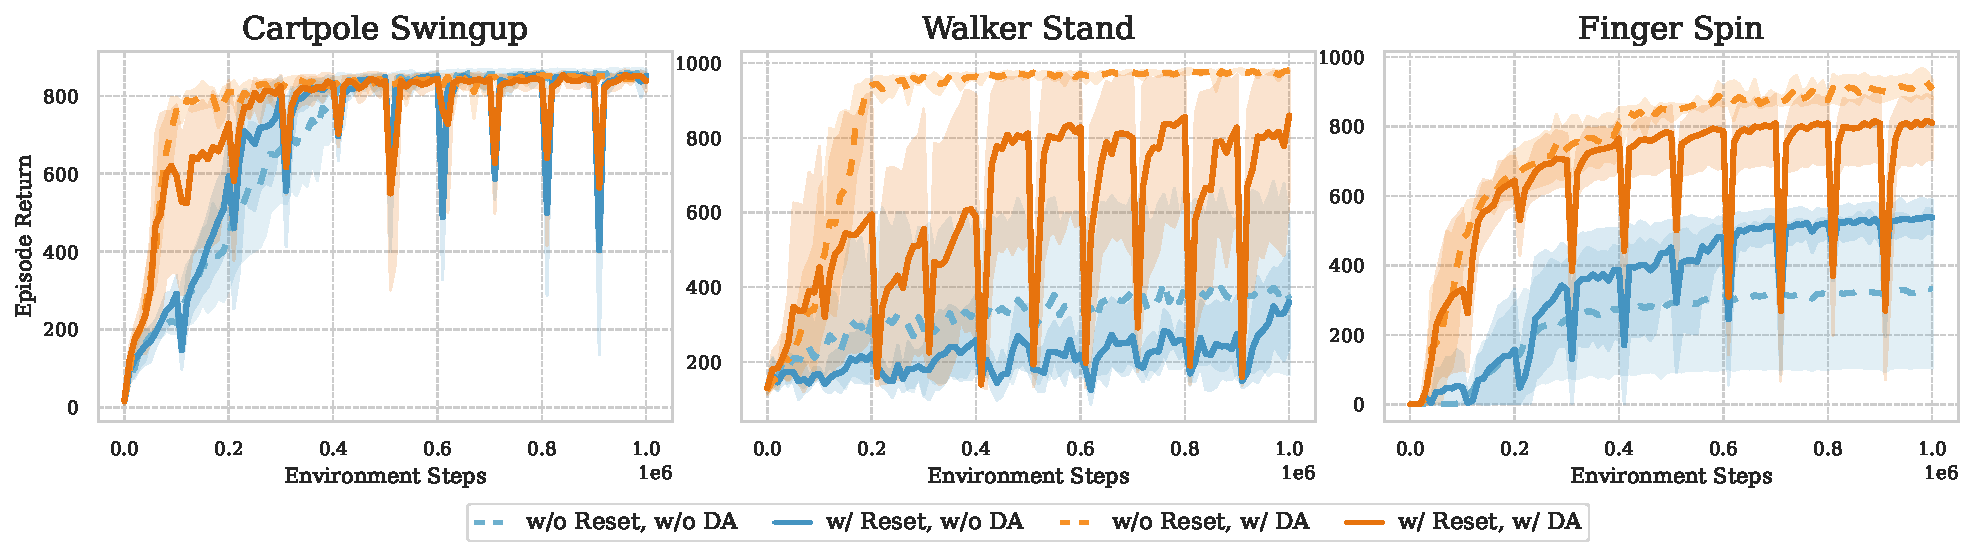
\includegraphics[width=\textwidth]{Figures/5Appendix/reset_DA_1M.pdf}
  \vspace{-2\baselineskip}
  \caption{Training curves across four combinations: incorporating or excluding Reset and DA.}
  % \vspace{-0.5\baselineskip}
  \label{appendix_fig:reset}
\end{figure}

\begin{figure}[ht]
  \centering
  % \vspace{-\baselineskip}
  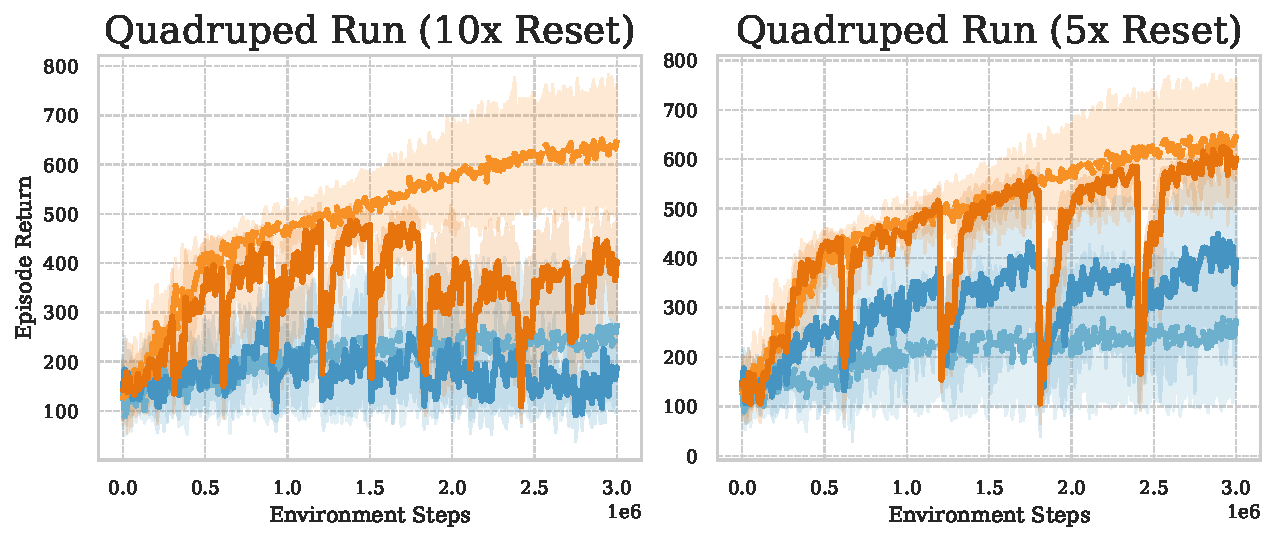
\includegraphics[width=0.6\textwidth]{Figures/5Appendix/reset_times_QR.pdf}
  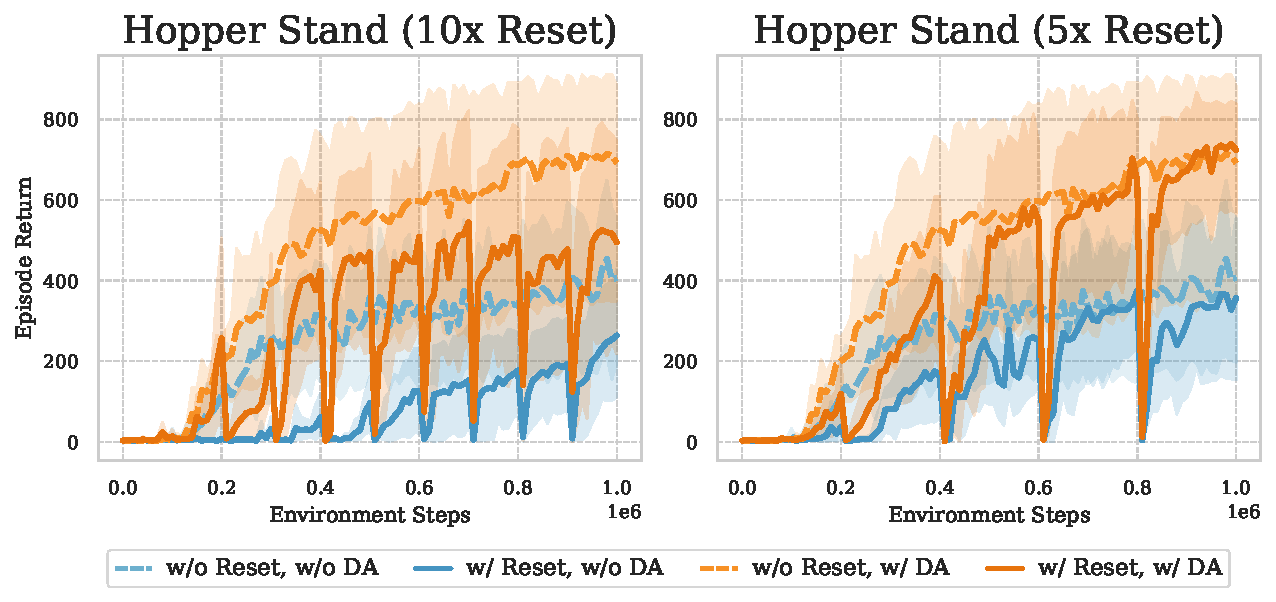
\includegraphics[width=0.6\textwidth]{Figures/5Appendix/reset_times.pdf}
  % \vspace{-\baselineskip}
  \caption{Learning curves for various reset intervals demonstrate that the effect of the reset strongly depends on the hyper-parameter that determines the reset interval.}
  % \vspace{-0.5\baselineskip}
  \label{appendix_fig:reset_interval}
\end{figure}

\newpage
\subsection{Heavy Priming Phenomenon}
\label{Appendix: Heavy Priming}

Heavy priming~\citep{primacy_bias} refers to updating the agent $10^5$ times using the replay buffer, which collects 2000 transitions after the start of the training process. Heavy priming can induce the agent to overfit to its early experiences. We conducted experiments to assess the effects of using heavy priming and DA, both individually and in combination. The training curves can be found in Figure~\ref{appendix_fig:heavy_priming}.
The findings indicate that, while heavy priming can markedly impair sample efficiency without DA, its detrimental impact is largely mitigated when DA is employed. Additionally, we examine the effects of employing DA both during heavy priming and subsequent training, as illustrated in Figure~\ref{appendix_fig:primingDA}. The results indicate that DA not only mitigates plasticity loss during heavy priming but also facilitates its recovery afterward.
\begin{figure}[ht]
  \centering
  % \vspace{-\baselineskip}
  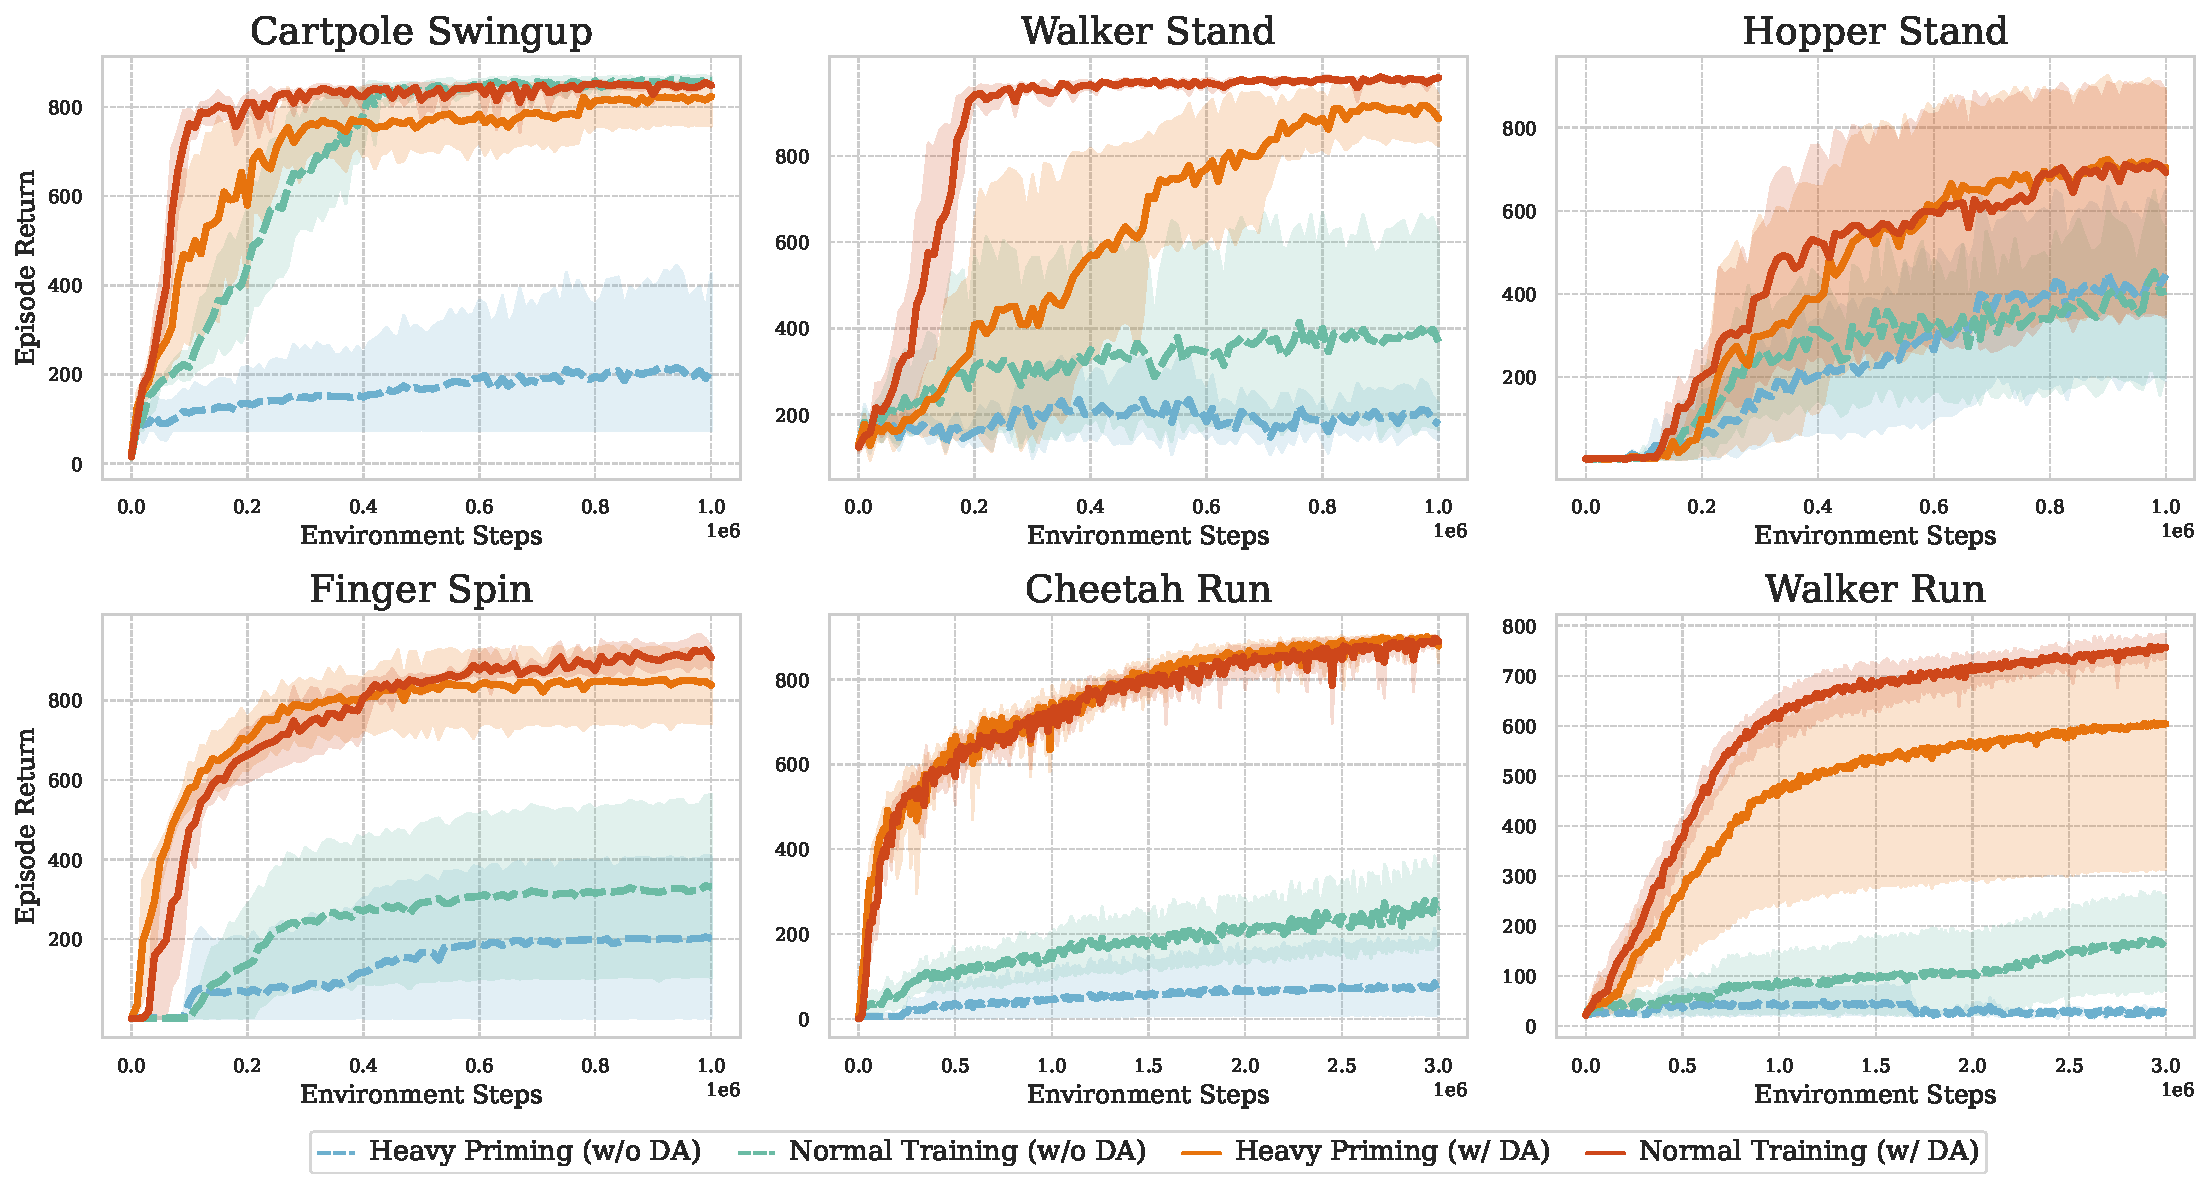
\includegraphics[width=\textwidth]{Figures/5Appendix/heavy_priming_vs_normal_training.pdf}
  \vspace{-\baselineskip}
  \caption{Heavy priming can severely damage the training efficiency when not employing DA.}
  % \vspace{-0.5\baselineskip}
  \label{appendix_fig:heavy_priming}
\end{figure}

\begin{figure}[ht]
  \centering
  % \vspace{-\baselineskip}
  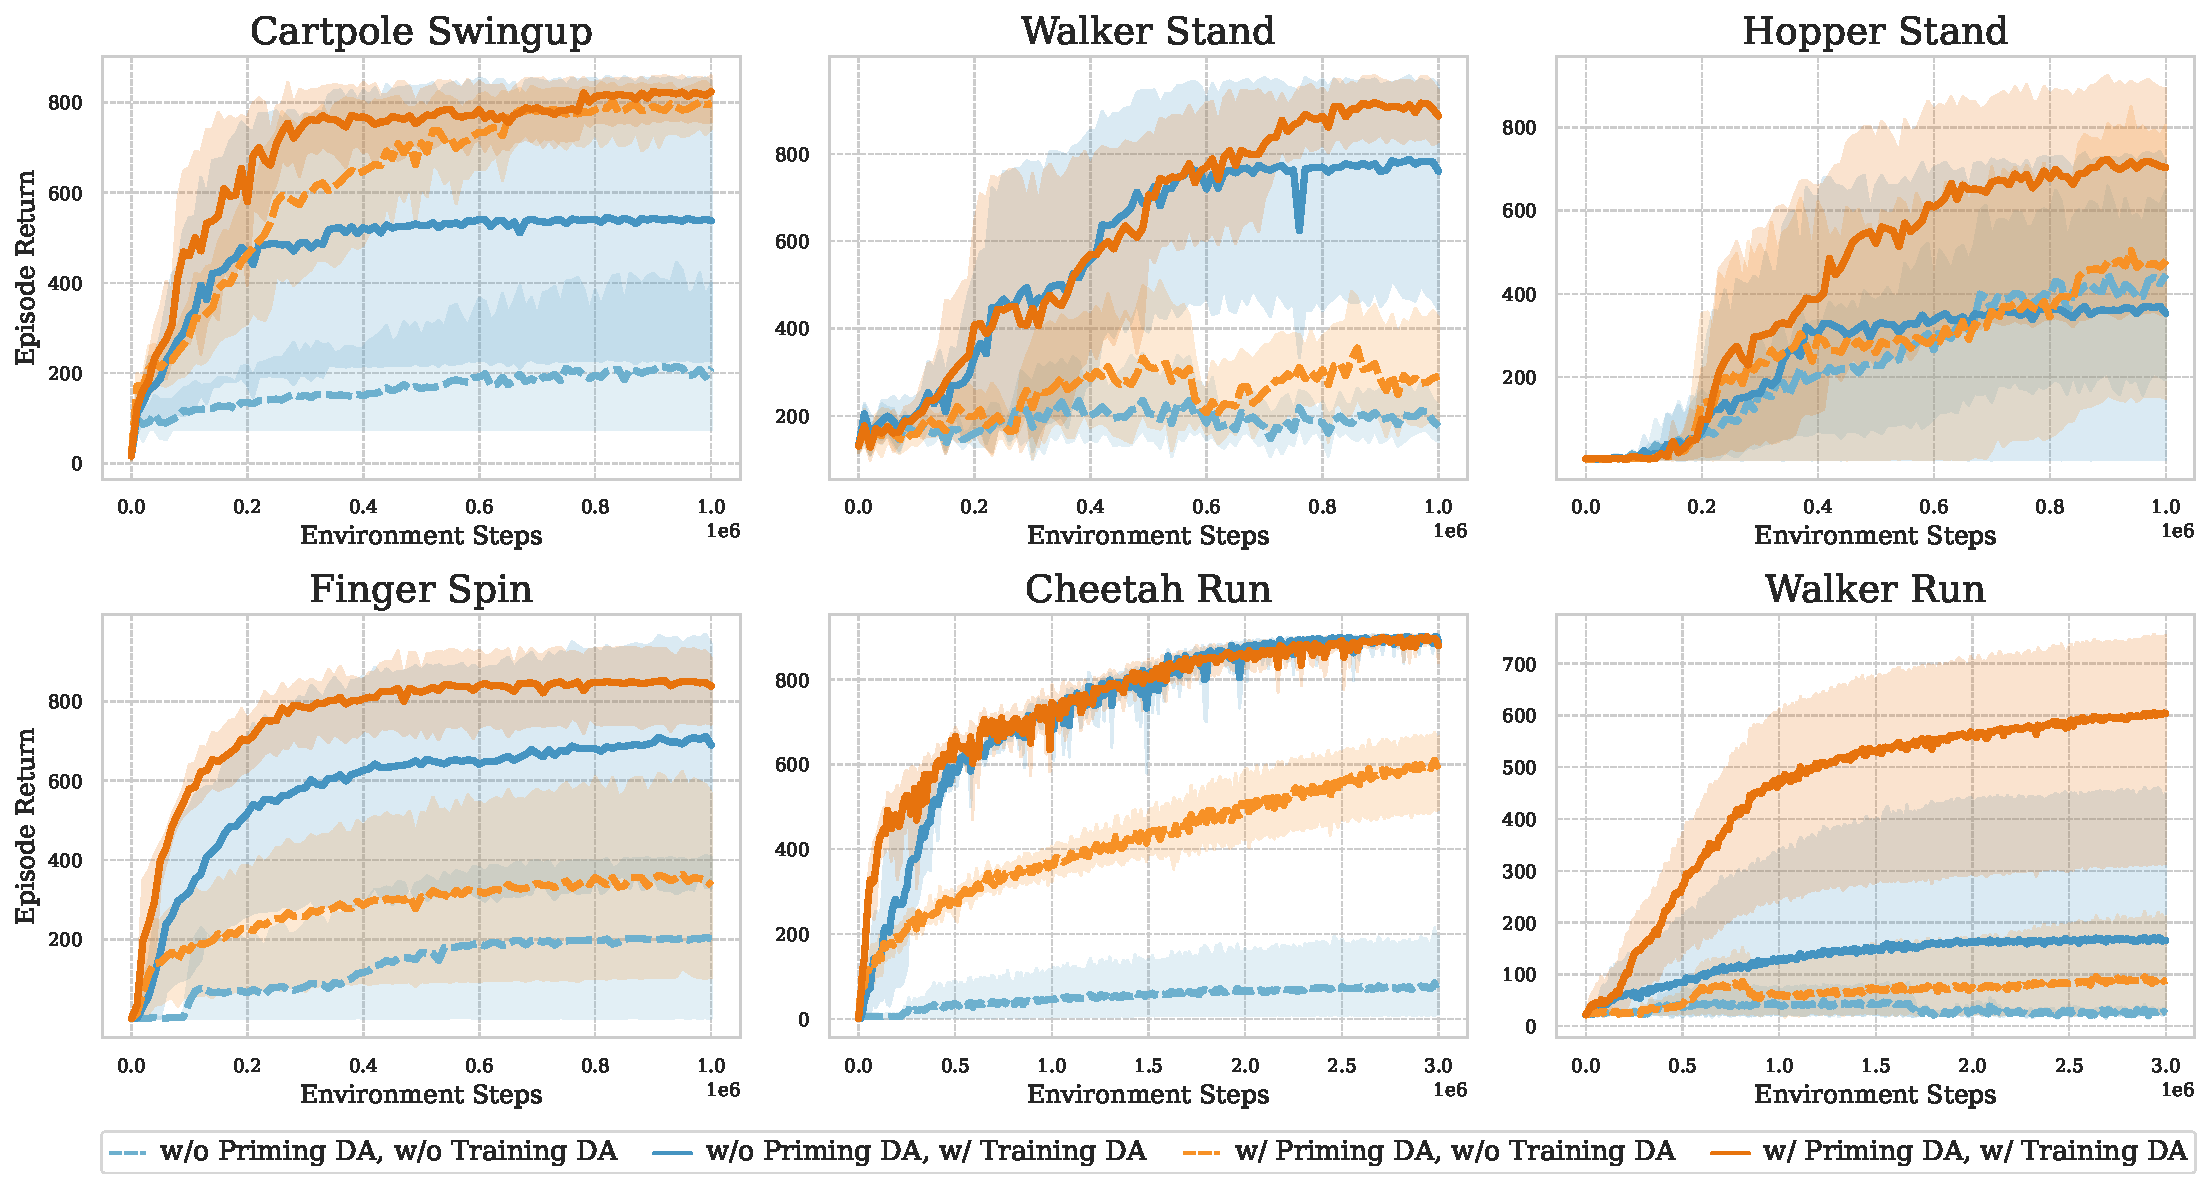
\includegraphics[width=\textwidth]{Figures/5Appendix/heavy_priming_DA.pdf}
  \vspace{-\baselineskip}
  \caption{DA not only can prevent the plasticity loss but also can recover the plasticity of agent after heavy priming phase.}
  \label{appendix_fig:primingDA}
\end{figure}

\subsection{Further Comparisons of DA with Other Interventions}
\label{Appendix: Further_Comparisons}

\begin{figure}[ht]
  \centering
  % \vspace{-\baselineskip}
  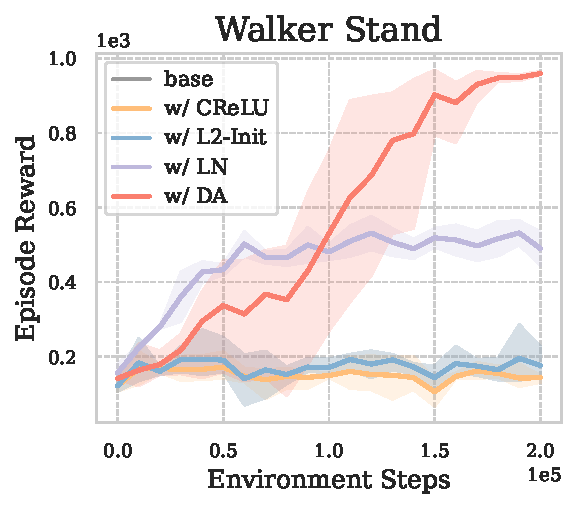
\includegraphics[width=0.4\textwidth]{Figures/5Appendix/Interventions_return.pdf}
  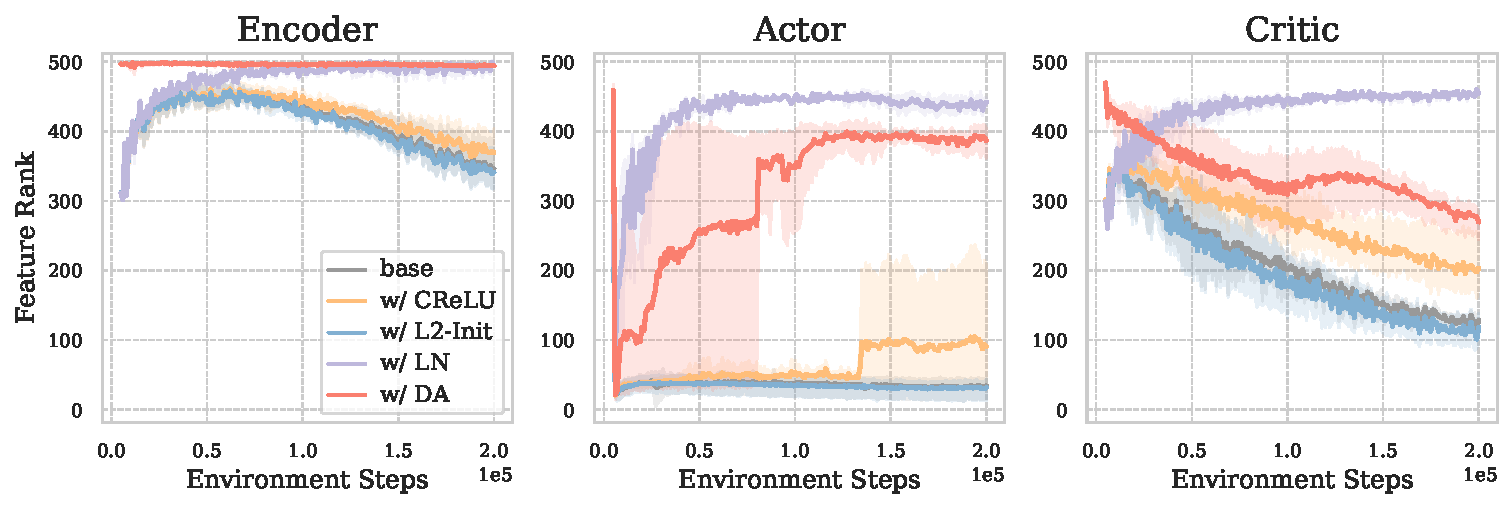
\includegraphics[width=\textwidth]{Figures/5Appendix/Interventions_Feature_Rank.pdf}
  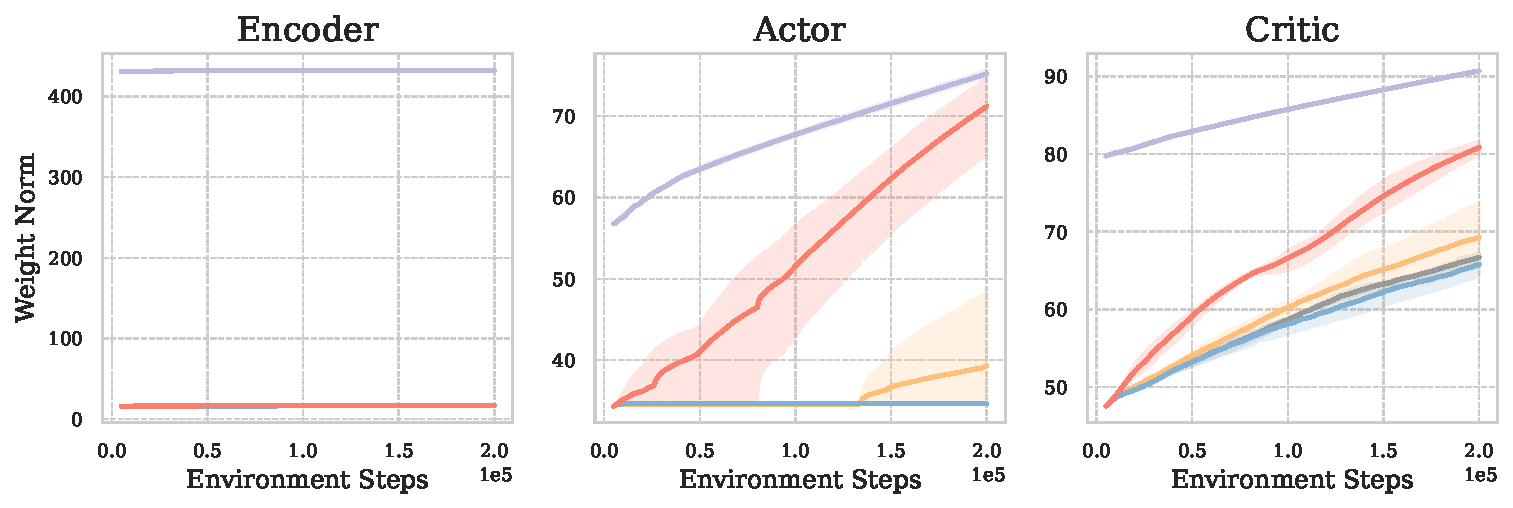
\includegraphics[width=\textwidth]{Figures/5Appendix/Interventions_WN.pdf}
  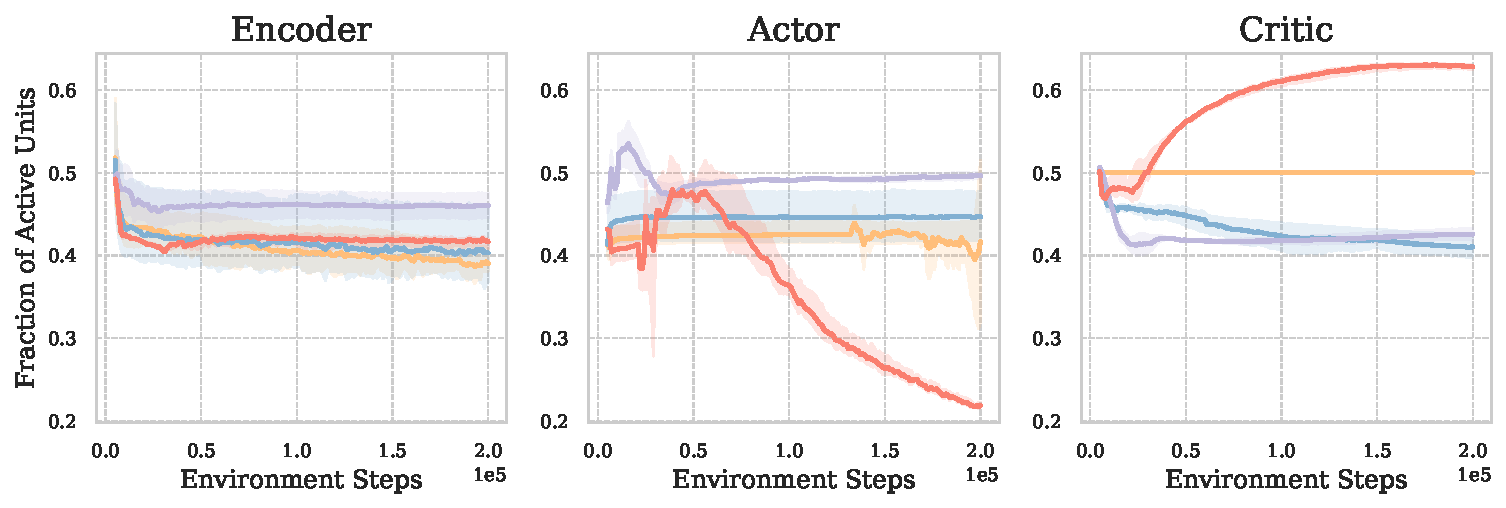
\includegraphics[width=\textwidth]{Figures/5Appendix/Interventions_FAU.pdf}
  \caption{We use three metrics - Feature Rank, Weight Norm, and Fraction of Active Units (FAU) - to assess the impact of various interventions on training dynamics.}
\end{figure}

\newpage
\subsection{Plasticity Injection}
\label{Appendix: Plasticity Injection}
\textit{Plasticity injection} is an intervention to increase the plasticity of a neural network. The network is schematically separated into an encoder $\phi(\cdot)$ and a head $h_{\theta}(\cdot)$. After plasticity injection, the parameters of head $\theta$ are frozen. Subsequently, two randomly initialized parameters, $\theta'_1$ and $\theta'_2$  are created. Here, $\theta'_1$ are trainable and $\theta'_2$ are frozen.
The output from the head is computed using the formula $h_{\theta}(z)+h_{\theta'_1}(z)-h_{\theta'_2}(z)$, where $z=\phi(x)$. 

We conducted additional plasticity injection experiments on Cheetah Run and Quadruped Run within DMC, as depicted in Figure~\ref{appendix_fig:Injection}. The results further bolster the conclusion made in Section~\ref{Sec: Modules}: critic’s plasticity loss is the primary culprit behind VRL’s sample inefficiency.
\begin{figure}[ht]
  \centering
  % \vspace{-\baselineskip}
  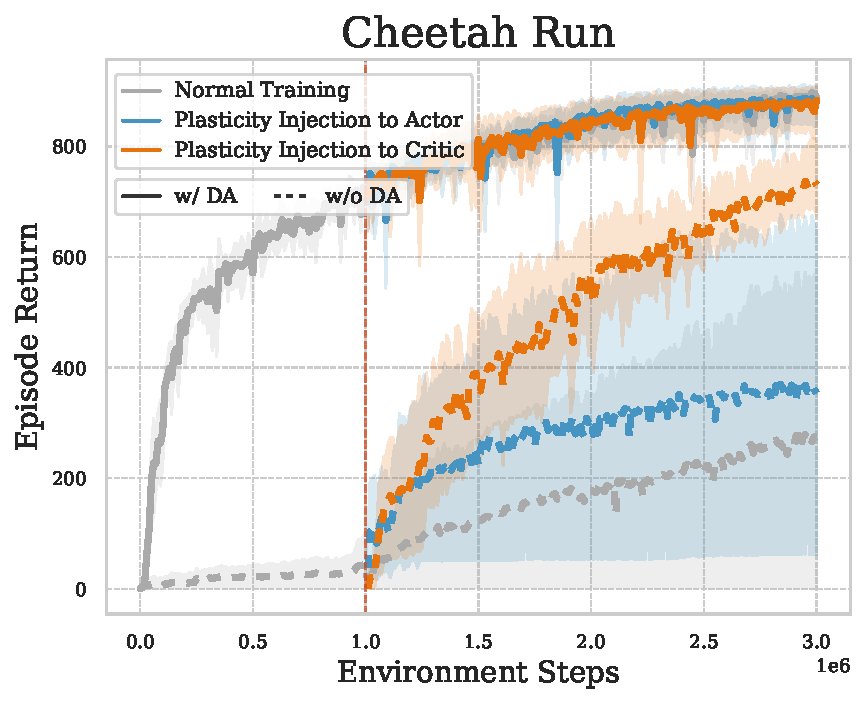
\includegraphics[width=0.49\textwidth]{Figures/5Appendix/Injection_CR.pdf}
  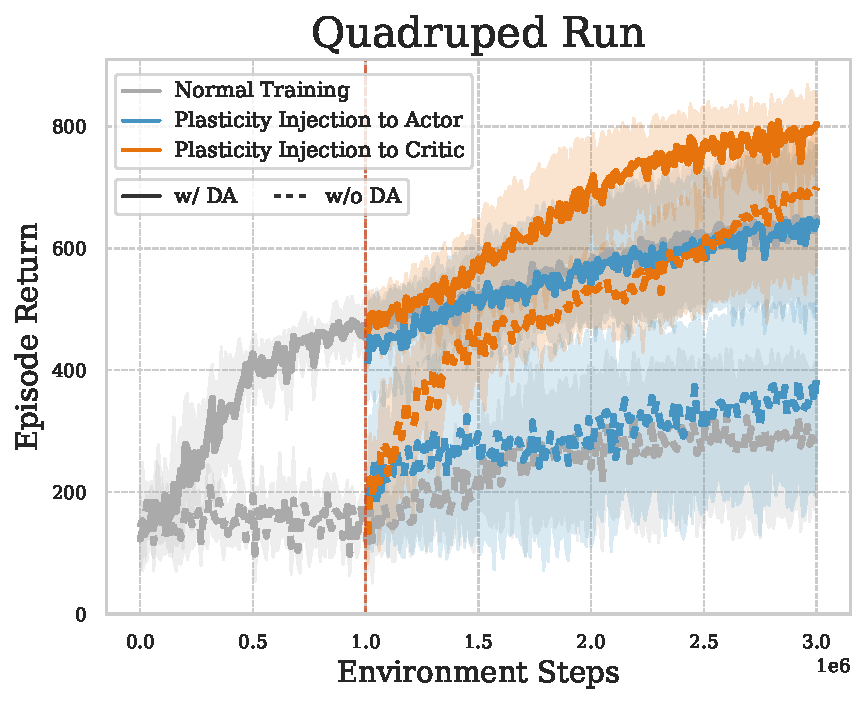
\includegraphics[width=0.49\textwidth]{Figures/5Appendix/Injection_QR.pdf}
  \vspace{-\baselineskip}
\caption{Training curves showcasing the effects of Plasticity Injection on either the actor or critic, evaluated on Cheetah Run and Quadruped Run.}

    \label{appendix_fig:Injection}
  % \vspace{-0.5\baselineskip}
\end{figure}

\subsection{Turning On or Turning off DA at Early Stages}
\label{Appendix: Turning DA}
In Figure~\ref{appendix_fig:turn_on_and_off_DA}, we present additional results across six DMC tasks for various DA application modes. As emphasized in Section~\ref{Sec: Stages}, it is necessary to maintain plasticity during early stages.
\begin{figure}[ht]
  \centering
  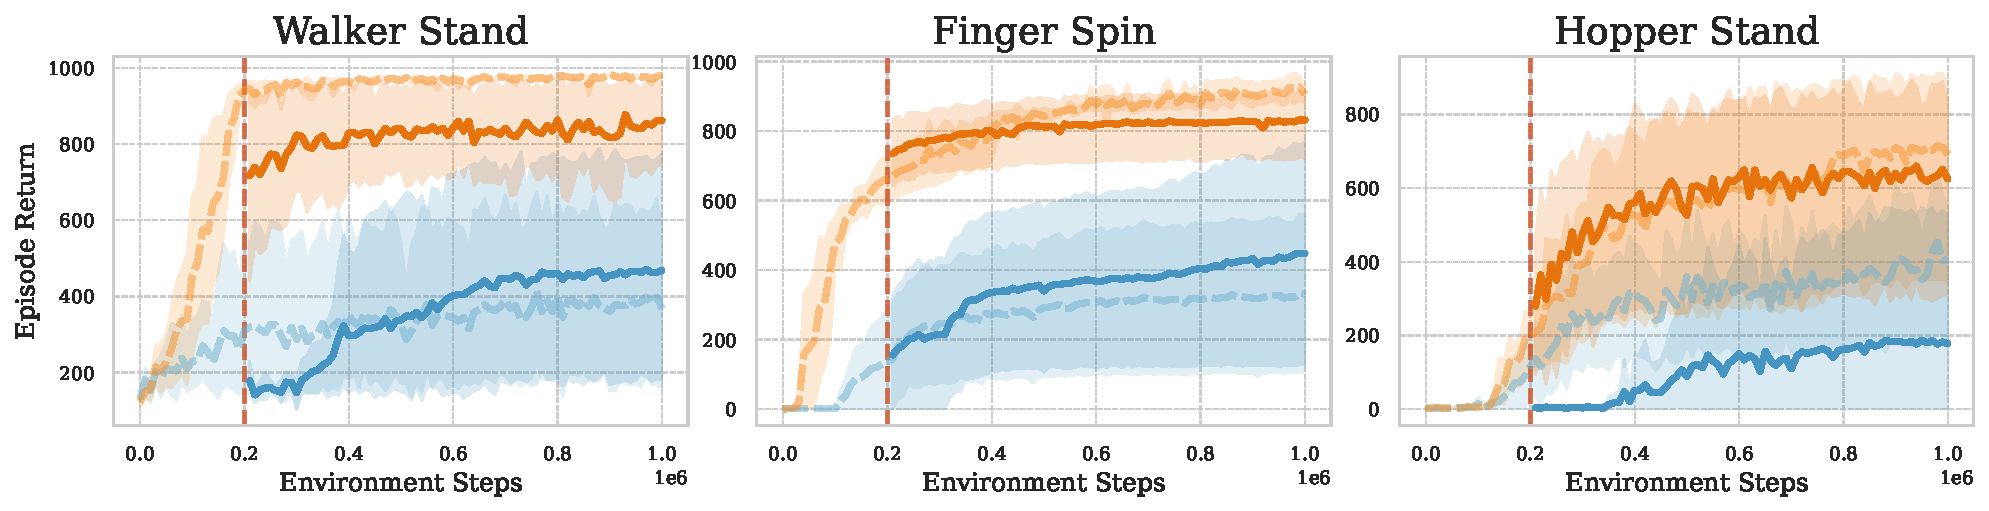
\includegraphics[width=\textwidth]{Figures/5Appendix/recover_WFH.pdf}
  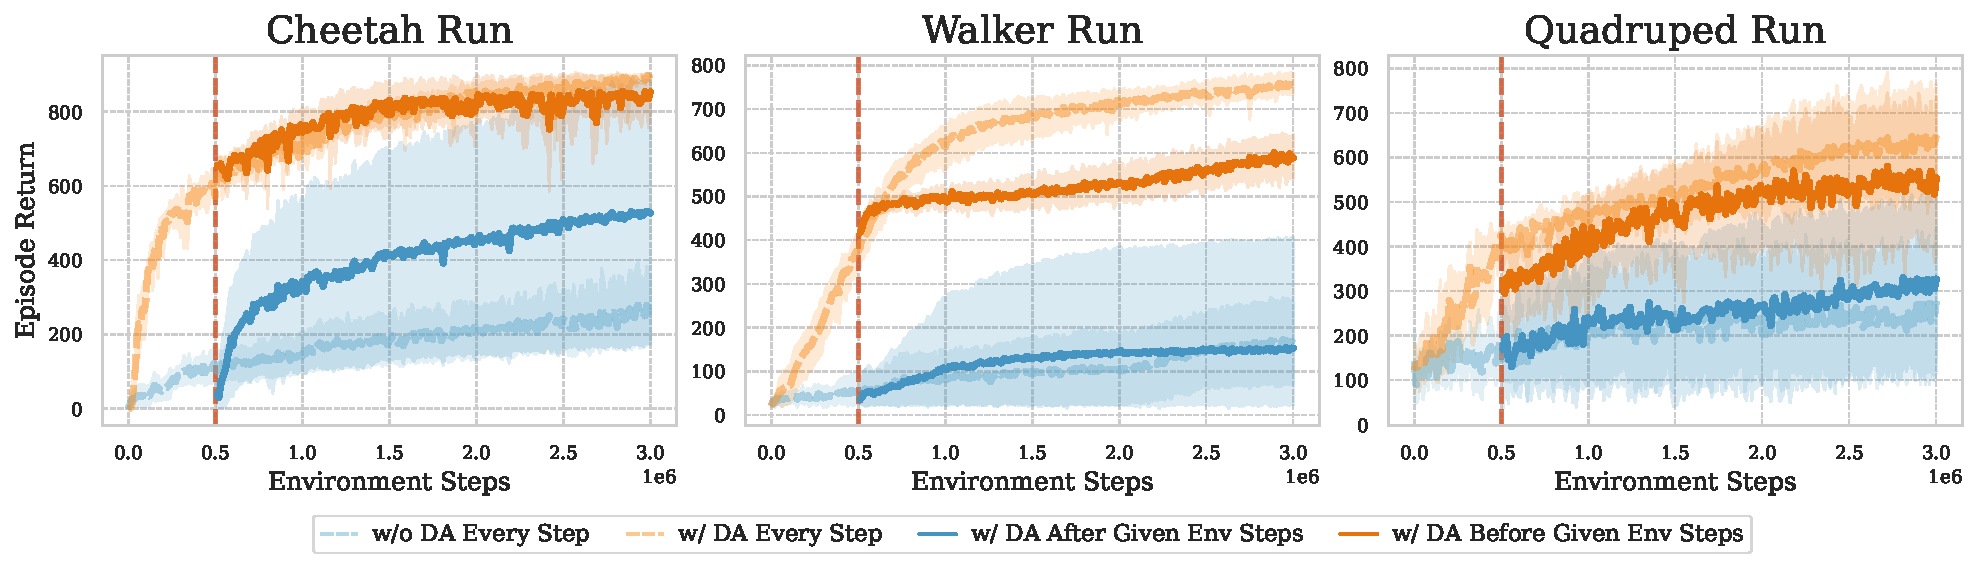
\includegraphics[width=\textwidth]{Figures/5Appendix/recover.pdf}
  \vspace{-\baselineskip}
  \caption{Training curves across different DA application modes, illustrating the critical role of plasticity in the early stage.}

  % \vspace{-0.5\baselineskip}
\label{appendix_fig:turn_on_and_off_DA}
\end{figure}

\newpage
\subsection{FAU Trends Across Different Tasks}
\label{Appendix: FAU trends}
In Figure~\ref{appendix_fig:FAU_task_1} and Figure~\ref{appendix_fig:FAU_task_2}, we showcase trends for various FAU modules across an additional nine DMC tasks as a complement to the main text. 
\begin{figure}[ht]
  \centering
  \vspace{2\baselineskip}
  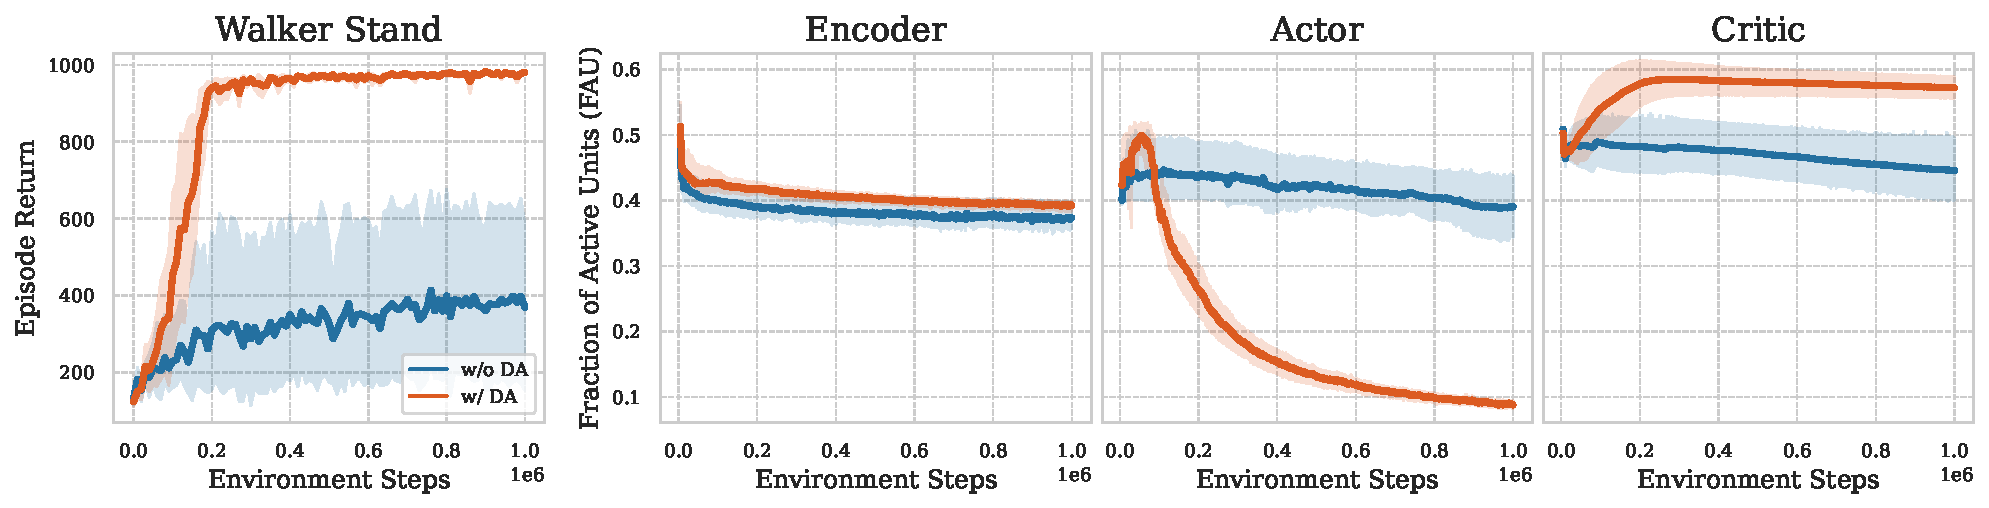
\includegraphics[width=\textwidth]{Figures/5Appendix/FAU_walker_stand.pdf}
  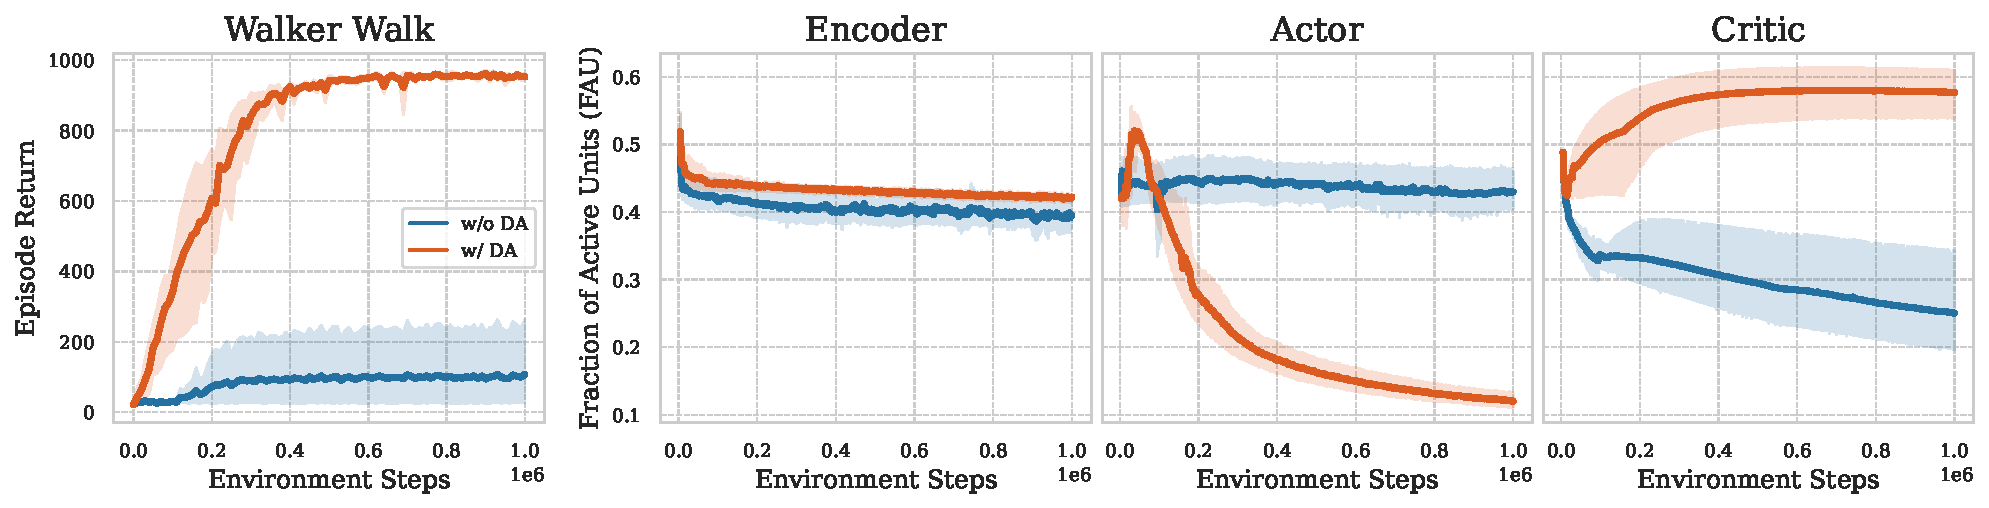
\includegraphics[width=\textwidth]{Figures/5Appendix/FAU_walker_walk.pdf}
  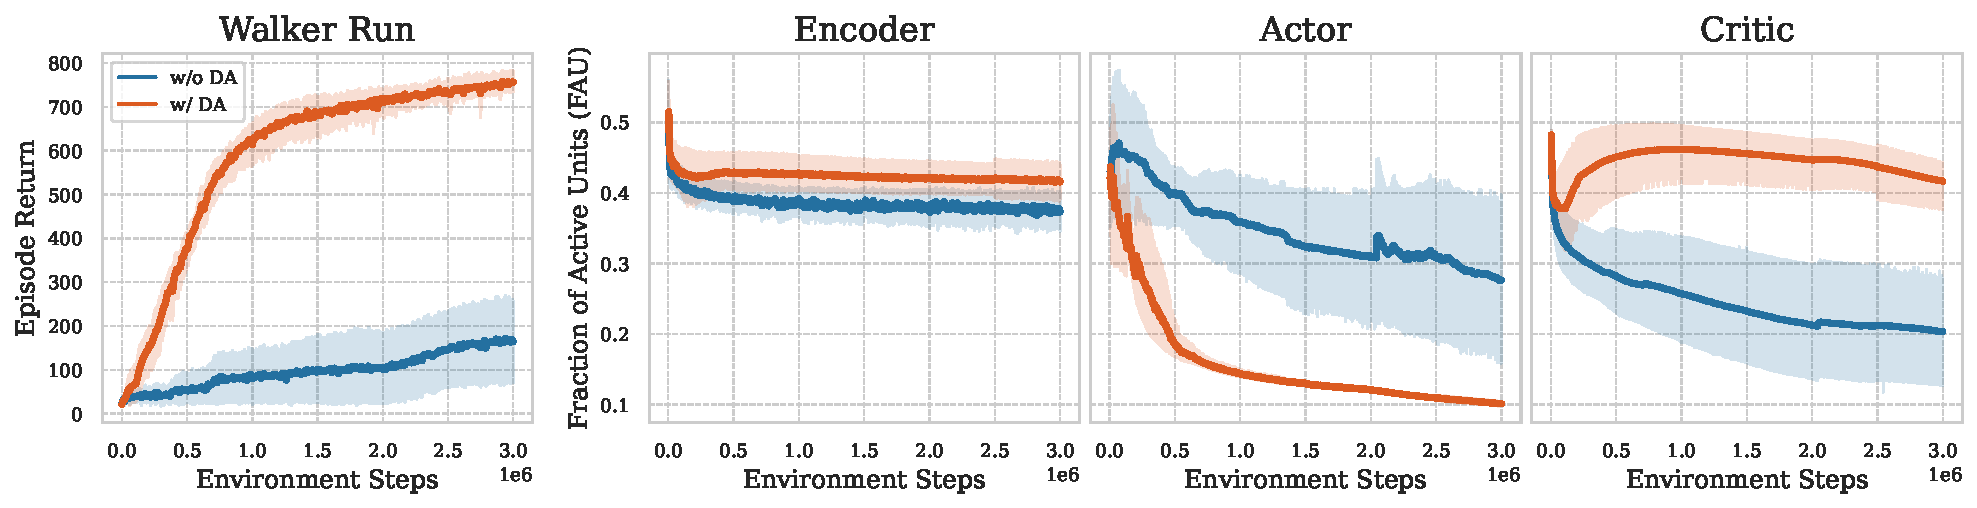
\includegraphics[width=\textwidth]{Figures/2Modules/FAU_walker_run.pdf}
  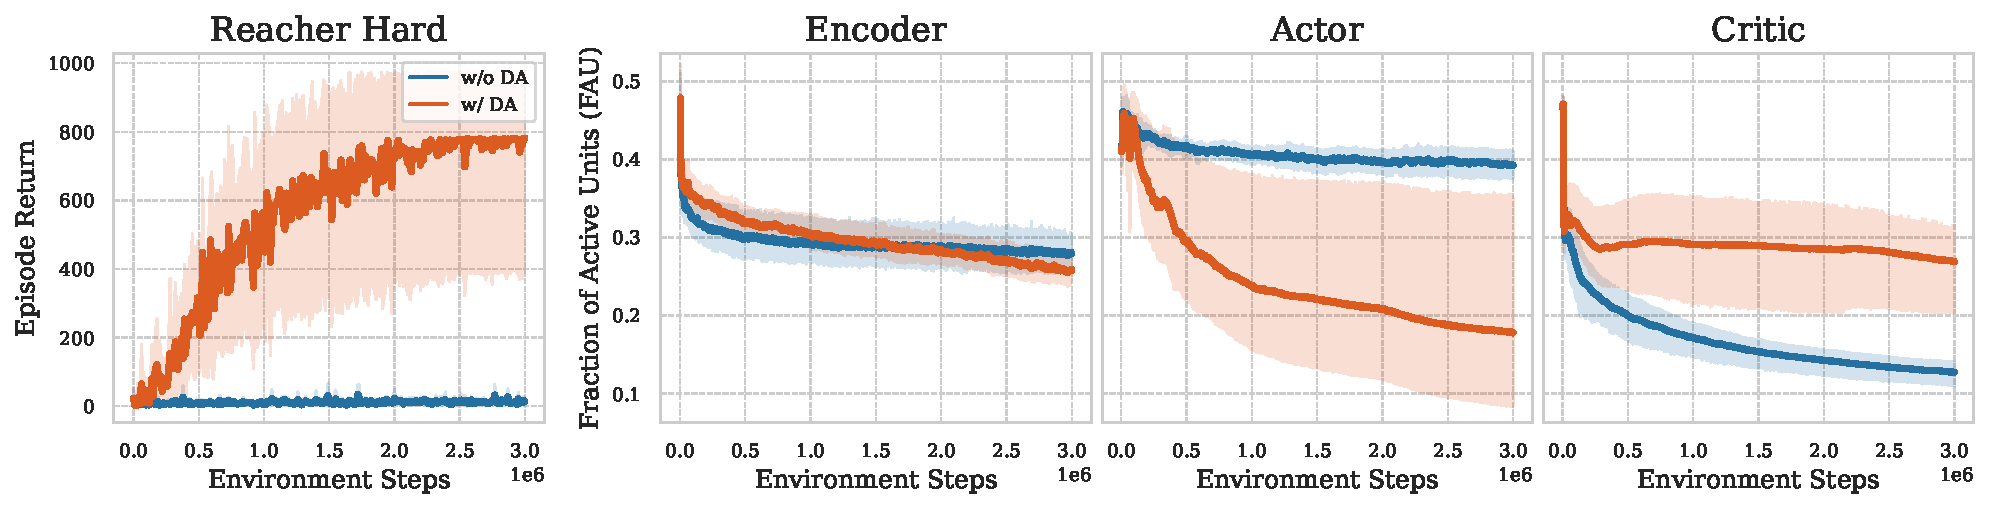
\includegraphics[width=\textwidth]{Figures/5Appendix/FAU_reacher_hard.pdf}
  \caption{FAU trends for various modules within the VRL agent across DMC tasks (\textit{Walker Stand}, \textit{Walker Walk}, \textit{Walker Run} and \textit{Reacher Hard}) throughout the training process.}
  % \vspace{-0.5\baselineskip}
  \label{appendix_fig:FAU_task_1}
\end{figure}

\newpage
\begin{figure}[ht]
  \centering
  \vspace{2\baselineskip}
  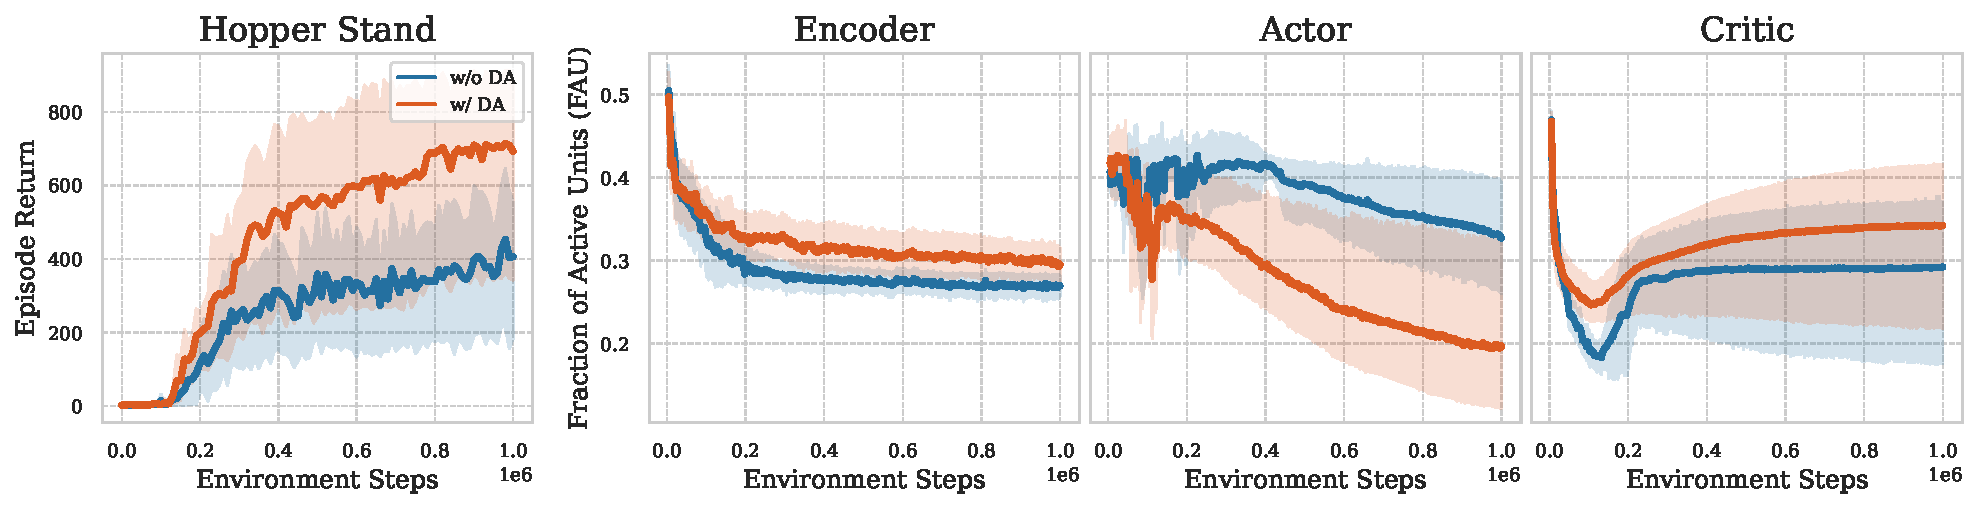
\includegraphics[width=\textwidth]{Figures/5Appendix/FAU_hopper_stand.pdf}
  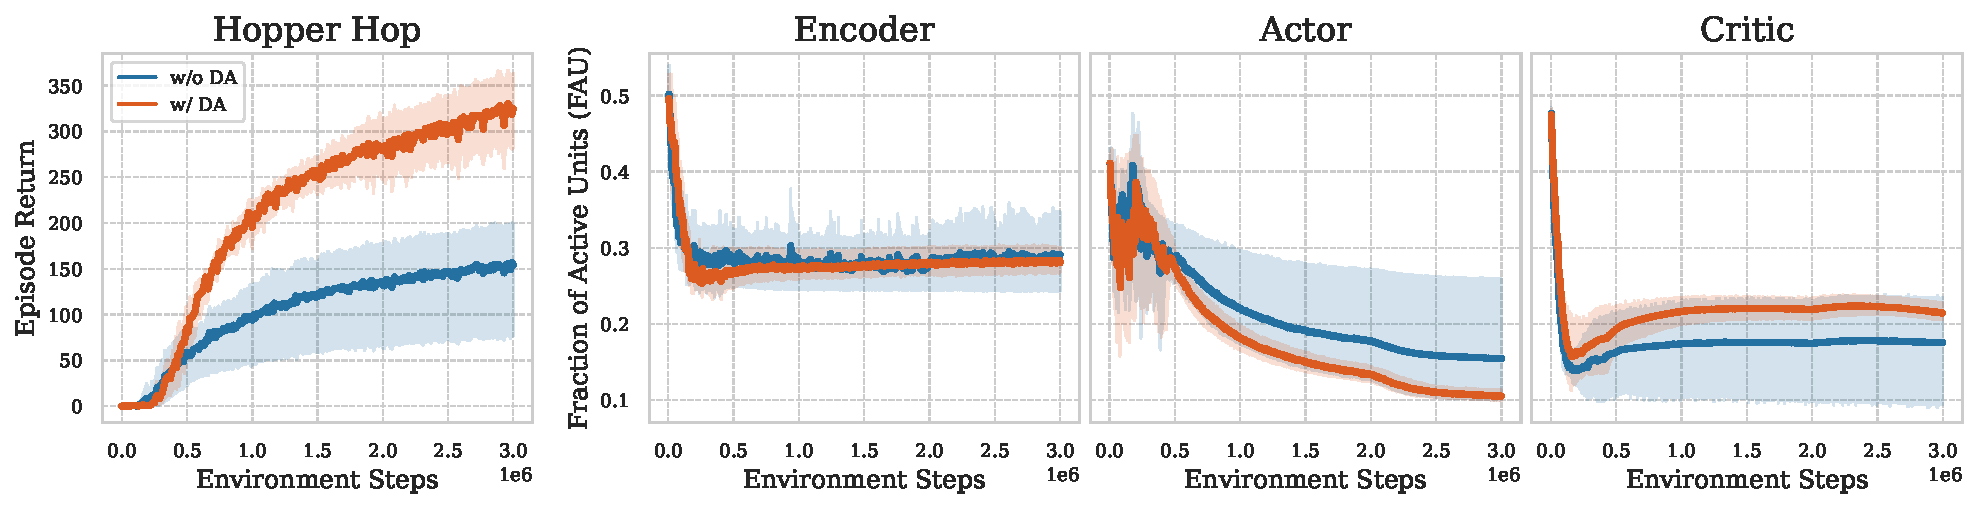
\includegraphics[width=\textwidth]{Figures/5Appendix/FAU_hopper_hop.pdf} 
  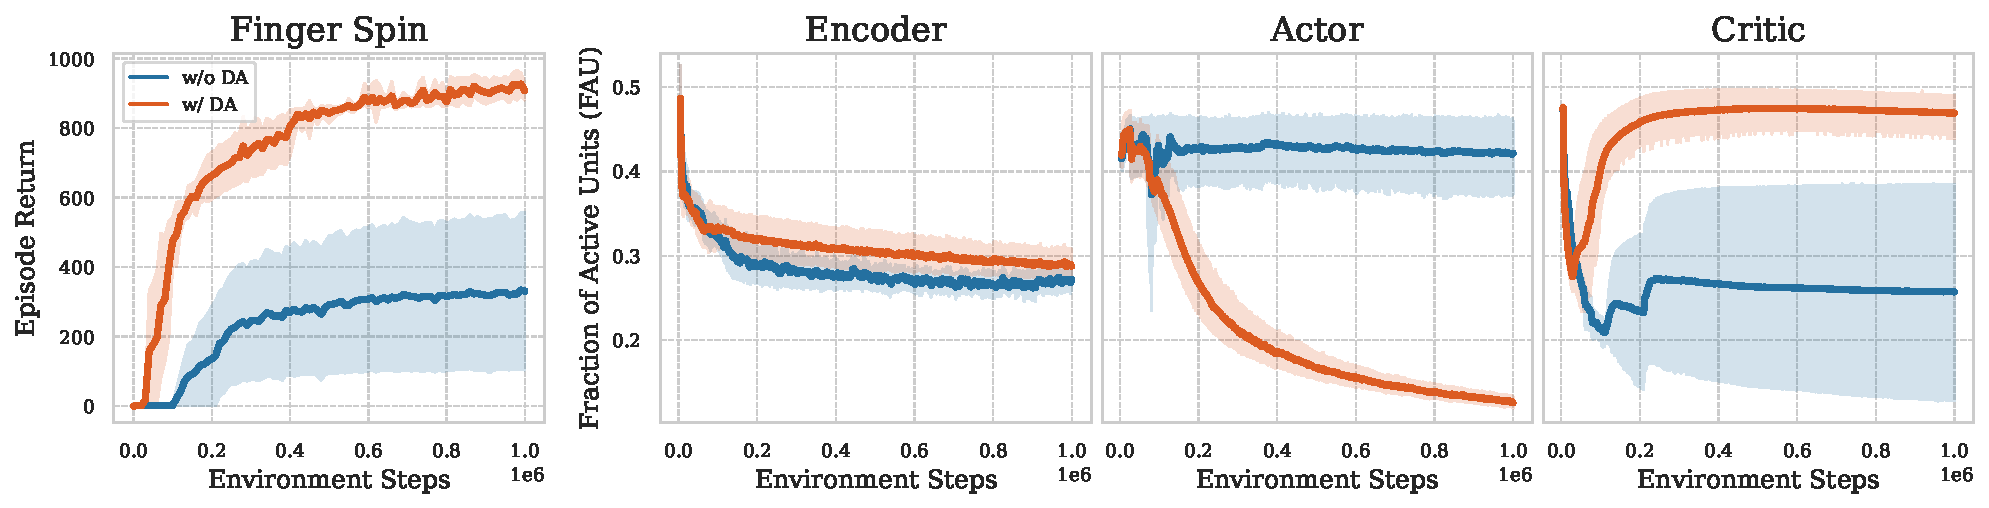
\includegraphics[width=\textwidth]{Figures/5Appendix/FAU_finger_spin.pdf}
  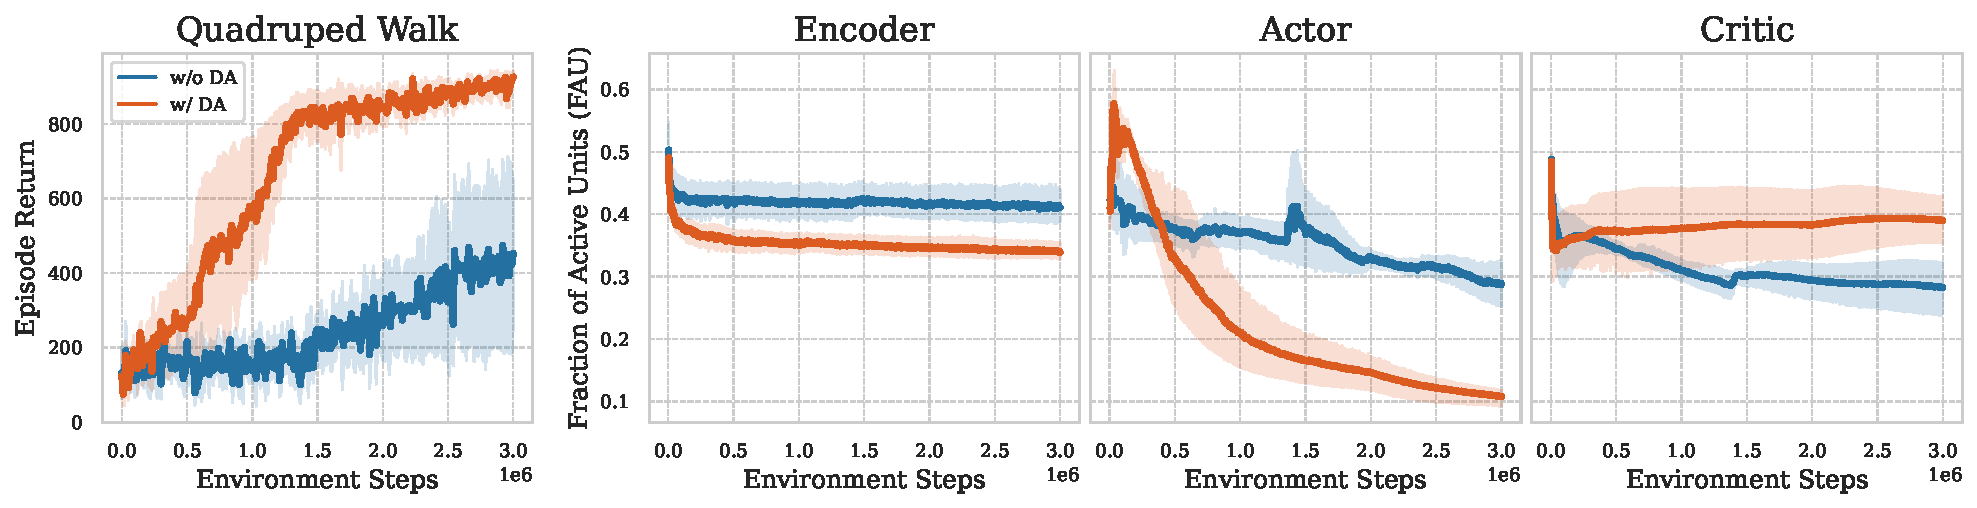
\includegraphics[width=\textwidth]{Figures/5Appendix/FAU_quadruped_walk.pdf}
  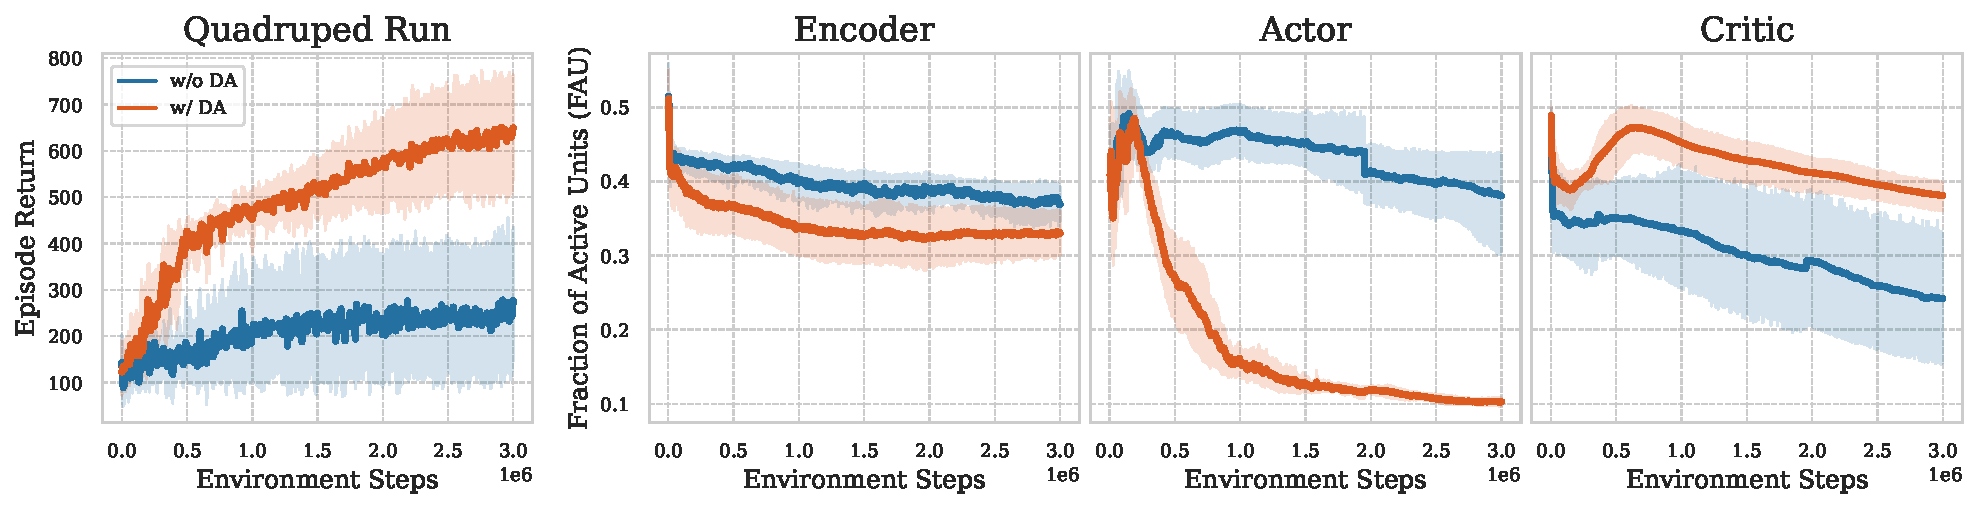
\includegraphics[width=\textwidth]{Figures/2Modules/FAU_quadruped_run.pdf}
  \caption{FAU trends for various modules within the VRL agent across DMC tasks (\textit{Hopper Stand}, \textit{Hopper Hop}, \textit{Finger Spin}, \textit{Quadruped Walk} and \textit{Quadruped Run}) throughout the training process.}
  % \vspace{-0.5\baselineskip}
  \label{appendix_fig:FAU_task_2}
\end{figure}

\newpage
Figure~\ref{appendix_fig:FAU_seed} provides the FAU for different random seeds, demonstrating that the trend is consistent across all random seeds.
\begin{figure}[ht]
  \centering
  % \vspace{-\baselineskip}
  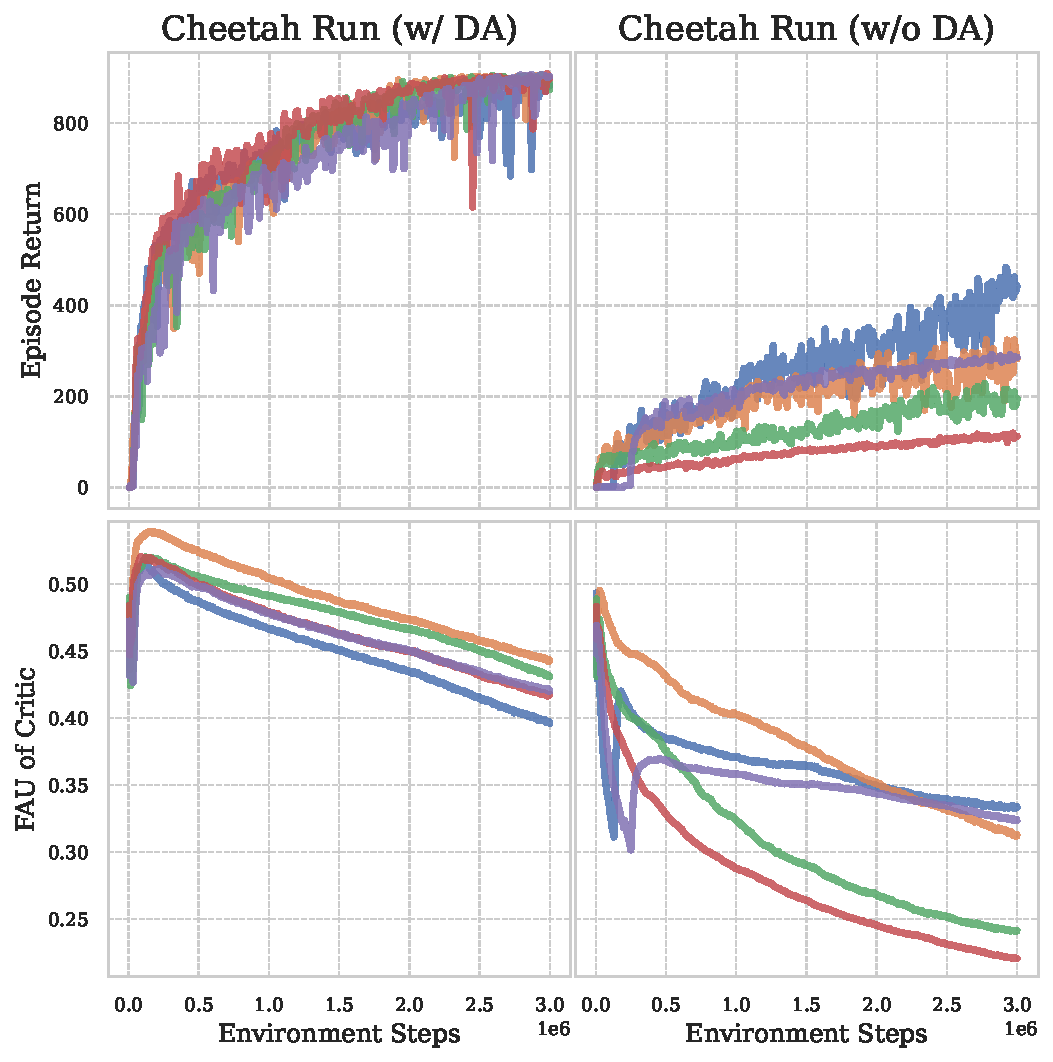
\includegraphics[width=0.45\textwidth]{Figures/5Appendix/sing_UTD_cheetah_run.pdf}
  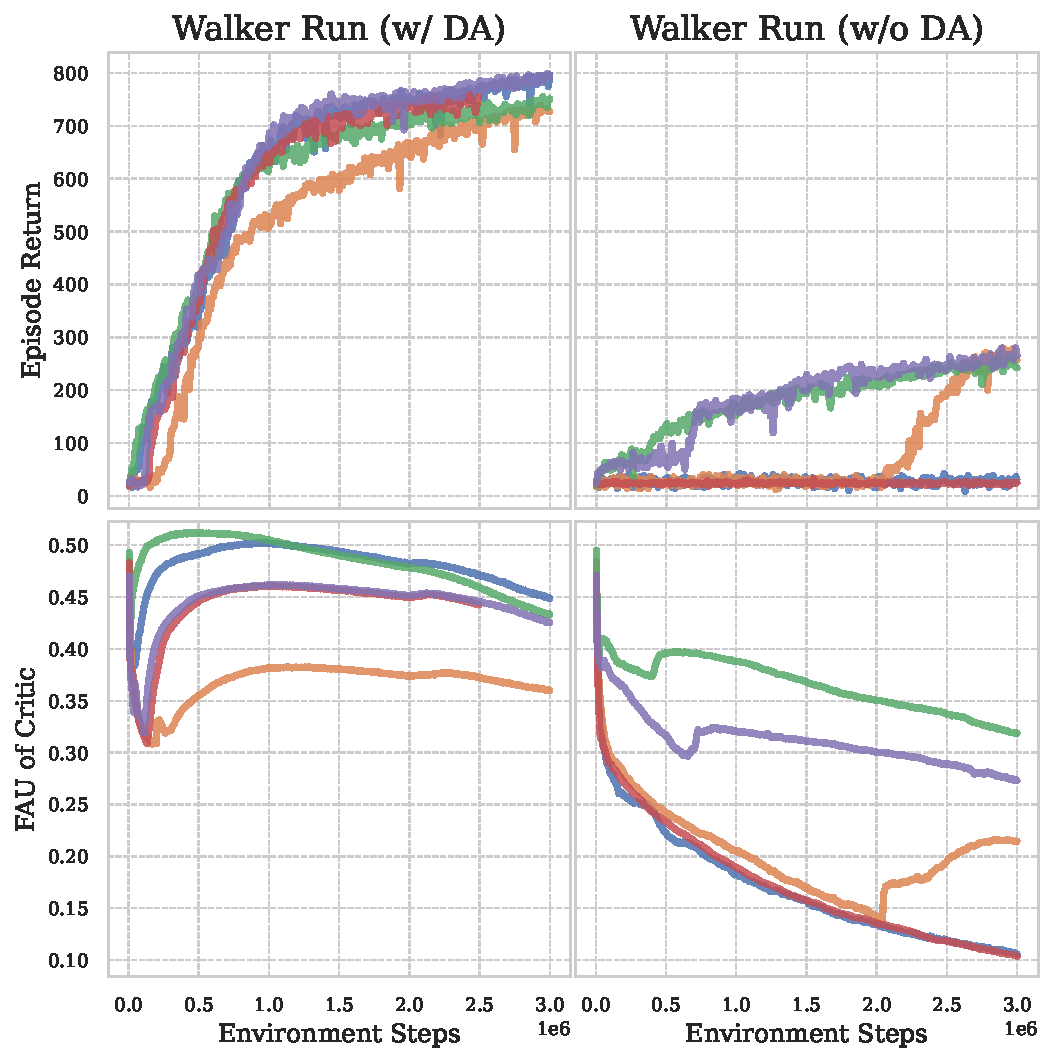
\includegraphics[width=0.45\textwidth]{Figures/5Appendix/sing_UTD_walker_run.pdf}
  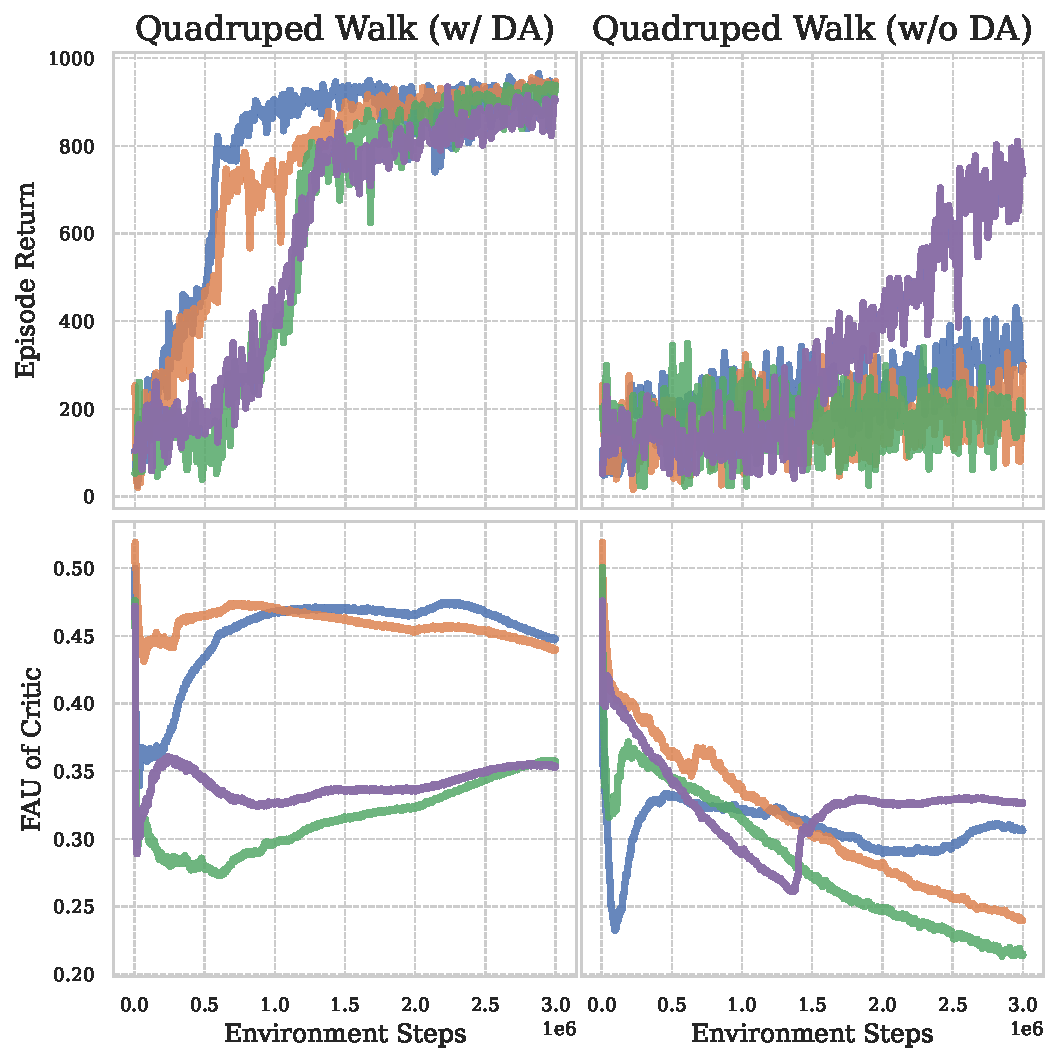
\includegraphics[width=0.45\textwidth]{Figures/5Appendix/sing_UTD_quadruped_walk.pdf}
  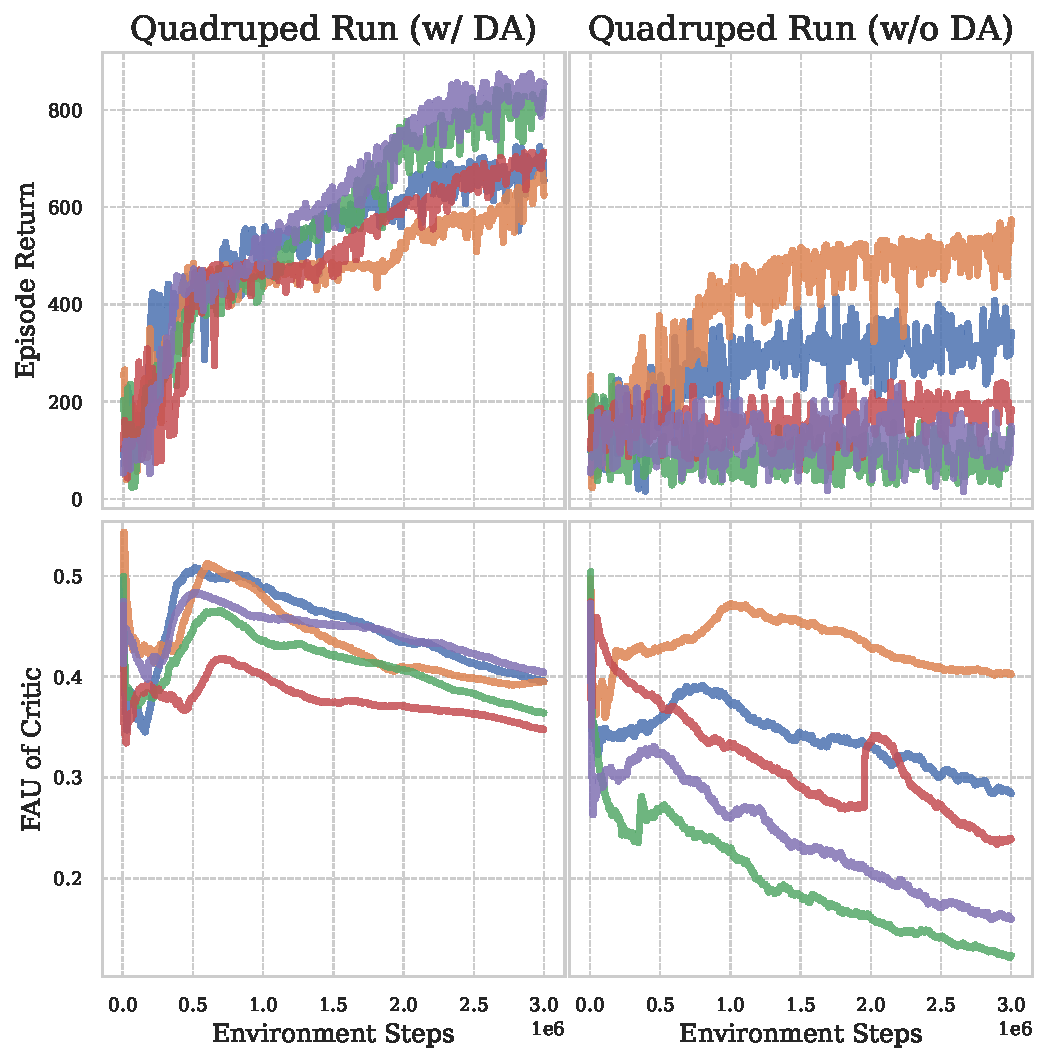
\includegraphics[width=0.45\textwidth]{Figures/5Appendix/sing_UTD_quadruped_run.pdf}
  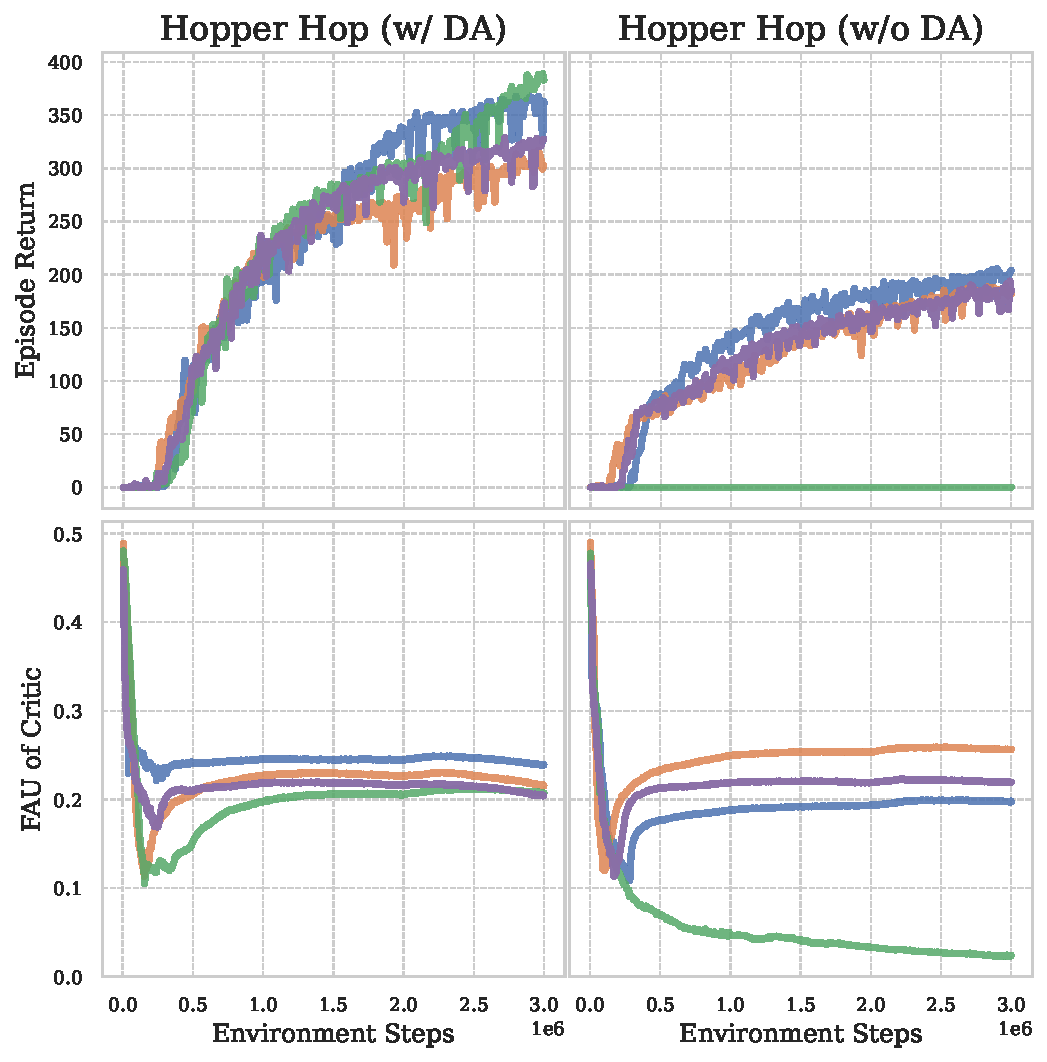
\includegraphics[width=0.45\textwidth]{Figures/5Appendix/sing_UTD_hopper_hop.pdf}
  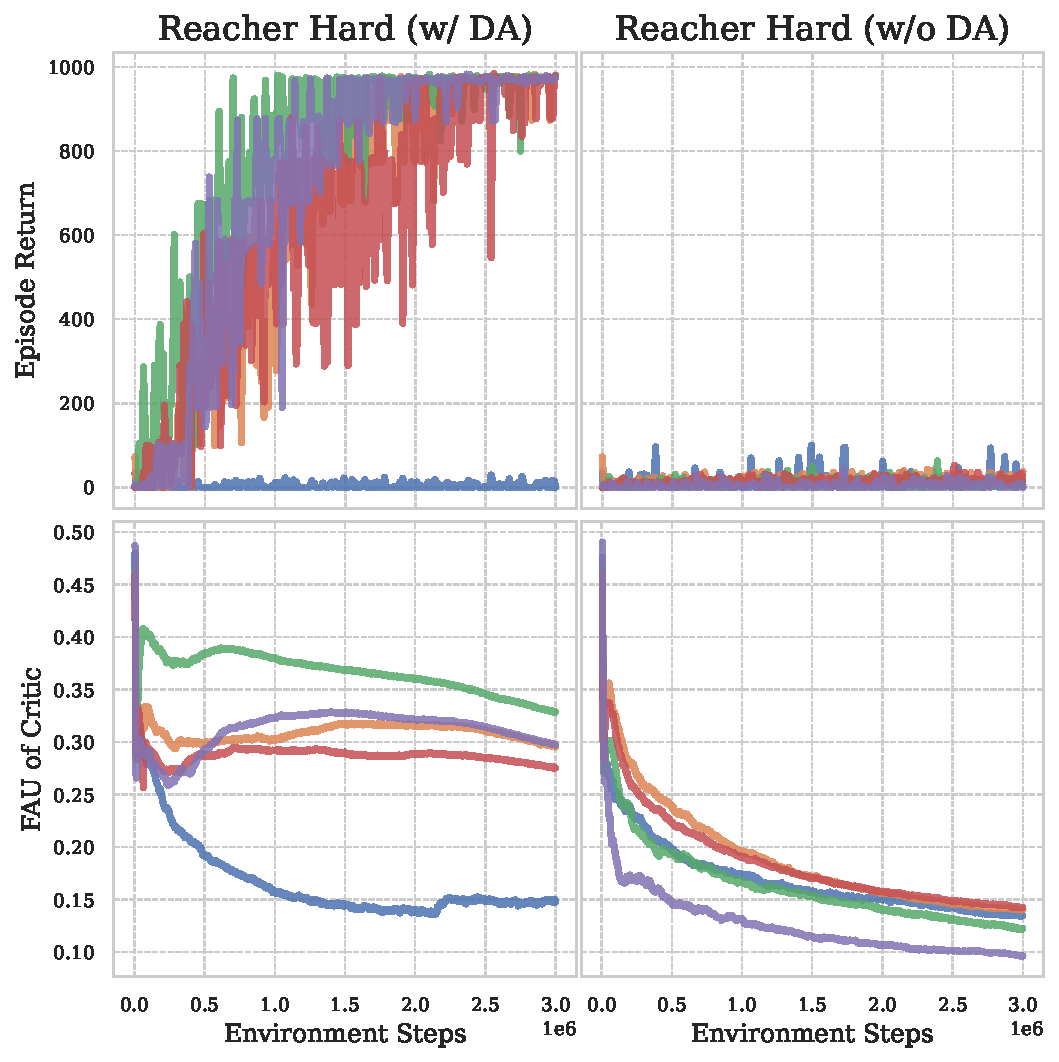
\includegraphics[width=0.45\textwidth]{Figures/5Appendix/sing_UTD_reacher_hard.pdf}
\caption{FAU trends for various modules within the VRL agent, evaluated across six DMC tasks and observed for each random seed throughout the training process.}
  % \vspace{-0.5\baselineskip}
  \label{appendix_fig:FAU_seed}
\end{figure}

\newpage
\subsection{Additional Metrics to Quantify the Plasticity}

\begin{figure}[ht]
  \centering
  % \vspace{-\baselineskip}
  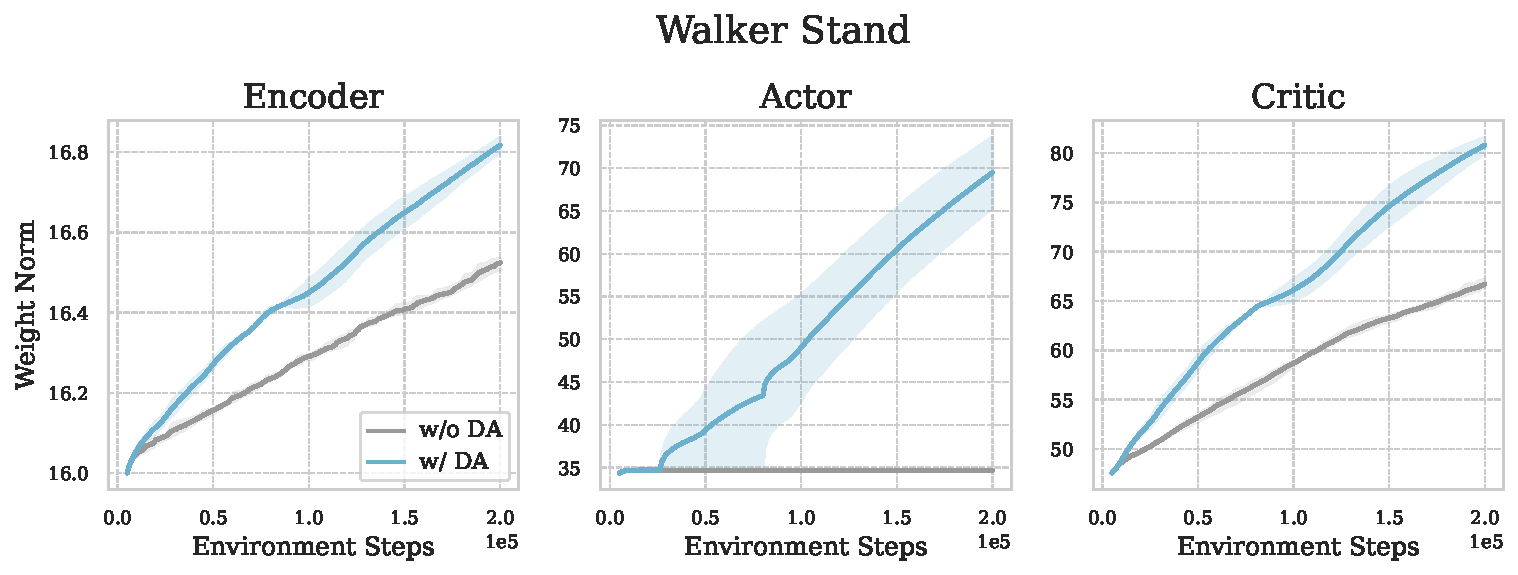
\includegraphics[width=0.9\textwidth]{Figures/5Appendix/WS_Weight_Norm.pdf}
  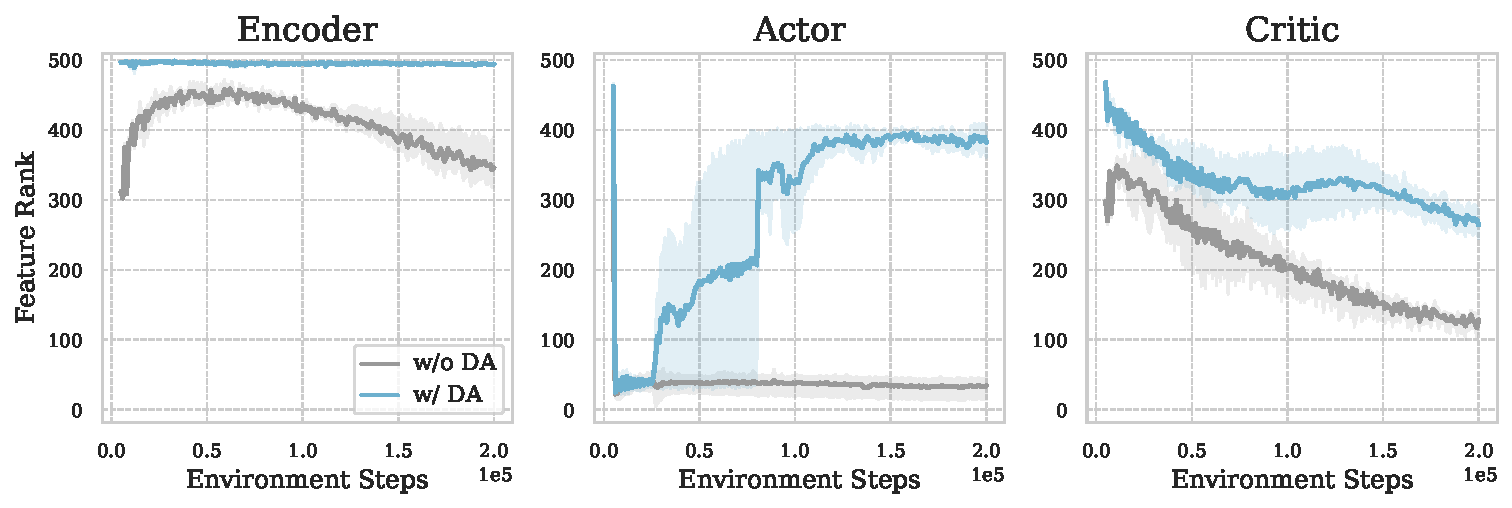
\includegraphics[width=0.9\textwidth]{Figures/5Appendix/WS_Feature_Rank.pdf}\\
  \vspace{\baselineskip} 
  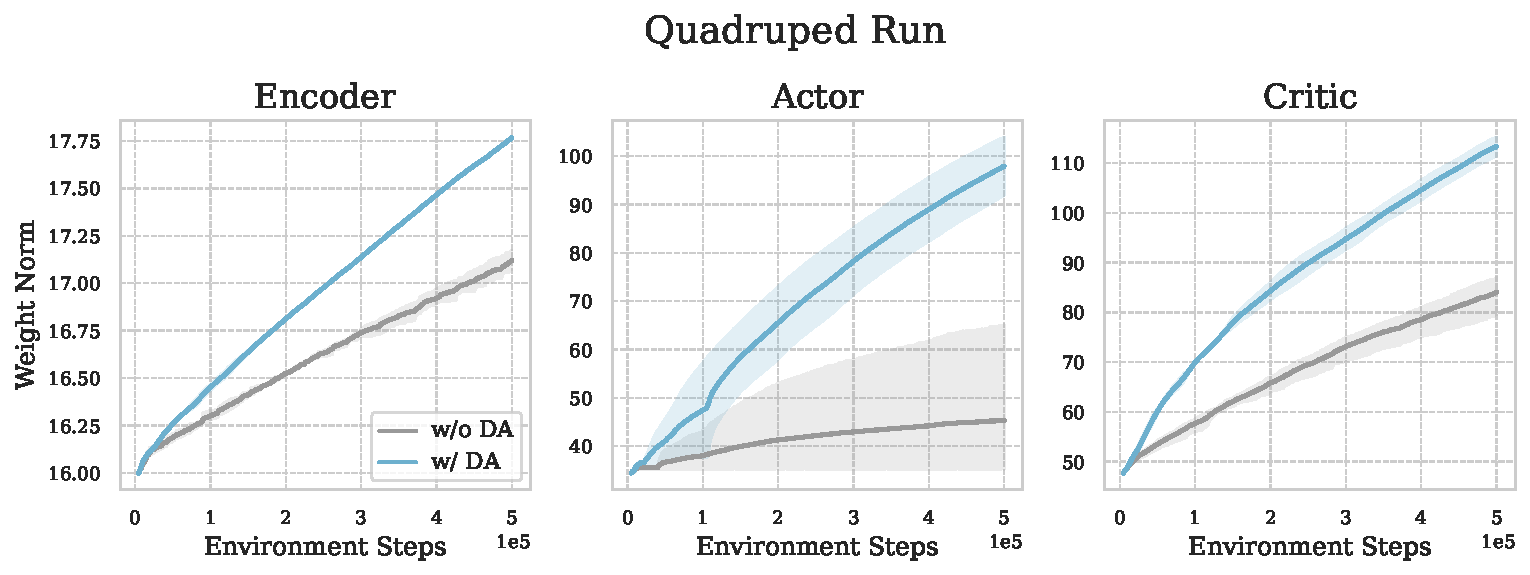
\includegraphics[width=0.9\textwidth]{Figures/5Appendix/QR_Weight_Norm.pdf}
  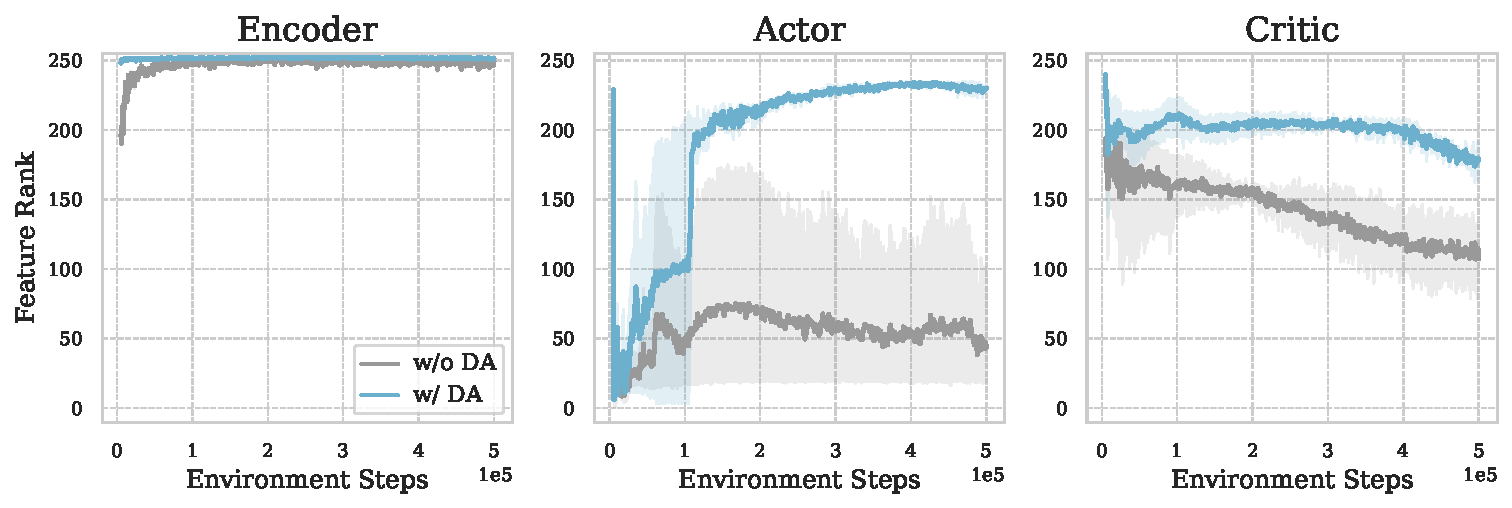
\includegraphics[width=0.9\textwidth]{Figures/5Appendix/QR_Feature_Rank.pdf}
  \caption{Measuring the plasticity of different modules via feature rank and weight norm.}
  % \vspace{-0.5\baselineskip}
  % \label{appendix_fig:FAU_task}
\end{figure}

\newpage
\section{Experimental Details}
In this section, we provide our detailed setting in experiments. 

\subsection{Algorithm}

\begin{center}
\begin{minipage}{.55\linewidth}
\begin{algorithm}[H]
 \caption{Adaptive RR}
  \begin{algorithmic}[1]
    \Require Check interval $I$, threshold $\tau$, total steps $T$
    \State Initialize RL training with a low RR
     \While{$t < T$} 
     %\Comment{Where $T$ is the total number of steps}
        \If{$t\%I=0$ and $|\Phi_{C}^{t} - \Phi_{C}^{t-I}|<\tau$}
            \State Switch to high RR 
        \EndIf
        \State Continue RL training with the current RR
        \State Increment step $t$
     \EndWhile
  \end{algorithmic}
  \label{algo:main}
\end{algorithm}
\end{minipage}
\end{center}

\subsection{DMC Setup}

We conducted experiments on robot control tasks within DeepMind Control using image input as the observation. All experiments are based on previously superior DrQ-v2 algorithms and maintain all hyper-parameters from DrQ-v2 unchanged. The only modification made was to the replay ratio, adjusted according to the specific setting.  The hyper-parameters are presented in Table \ref{table:DMC}.
\begin{table}[htbp] 
\caption{ A default set of hyper-parameters used in DMControl evaluation.}
\renewcommand{\arraystretch}{1.15}
\centering
\begin{tabular}{lc}
\toprule
\multicolumn{2}{c}{Algorithms Hyper-parameters} \\
\midrule
Replay buffer capacity & $10^6$ \\
Action repeat & $2$ \\
Seed frames & $4000$ \\
Exploration steps & $2000$ \\
$n$-step returns & $3$ \\
Mini-batch size & $256$ \\
Discount $\gamma$ & $0.99$ \\
Optimizer & Adam \\
Learning rate & $10^{-4}$ \\
Critic Q-function soft-update rate $\tau$ & $0.01$ \\
Features dim. & $50$ \\
Repr. dim. & $32 \times 35 \times 35$ \\
Hidden dim. & $1024$ \\
Exploration stddev. clip & $0.3$ \\
Exploration stddev. schedule & $\mathrm{linear}(1.0, 0.1, 500000)$\\ 
\bottomrule
\end{tabular}
\label{table:DMC}
\end{table}

\newpage
\section{Evaluation on Atari}
\label{Evaluation on Atari}

\textbf{Implement details.} Our Atari experiments and implementation were based on the Dopamine framework~\citep{castro18dopamine}. For ReDo~\citep{dormant_neuron} and DrQ($\epsilon$), We used the same setting as Dopamine, shown in Table~\ref{table:atari-config}. we use 5 independent random seeds for each Atari game. The detailed results are shown in Table~\ref{table:atari-full}.

\begin{table}[ht]
\caption{Hyper-parameters for Atari-100K.}
\label{table:common_hyperparameters}
\vspace{-\baselineskip}
\begin{center}
\begin{tabular}{lr}
\toprule
Common Parameter-DrQ($\epsilon$)& Value \\
\midrule
Optimizer & Adam \\
Optimizer: Learning rate &  $1 \times 10^{-4}$ \\
Optimizer: $\epsilon$ & $1.5 \times 10^{-4}$ \\
Training $\epsilon$ & 0.01 \\
Evaluation $\epsilon$ & 0.001 \\
Discount factor & 0.99 \\
Replay buffer size & $10^6$ \\
Minibatch size & 32 \\
Q network: channels & 32, 64, 64 \\
Q-network: filter size & 8 $\times$ 8, 4 $\times$ 4, 3 $\times$ 3 \\
Q-network: stride & 4, 2, 1 \\ 
Q-network: hidden units &  512 \\
Initial collect steps & 1600 \\
$n$-step & 10 \\
Training iterations & 40 \\
Training environment steps per iteration & 10K \\
   \toprule
 ReDo Parameter& Value\\
\hline
Recycling period & 1000 \\
$\tau$-Dormant  & 0.025\\ 
%for default setting, 0.1 otherwise\\
Minibatch size for estimating neurons score & 64\\
 \toprule
 Adaptive RR Parameter & Value \\
   \hline
 check interval & 2000\\
 threshold & 0.001\\
 low Replay Ratio & 0.5 \\
 high Replay Ratio & 2\\

\bottomrule
\end{tabular}
\end{center}
\label{table:atari-config}
\vskip -0.1in
\end{table}


\begin{table}[ht]
\centering
\caption{\textbf{Evaluation of Sample Efficiency on Atari-100k.} We report the scores and the mean and median HNSs achieved by different methods on Atari-100k.}
\renewcommand{\arraystretch}{1.15}
\begin{small}
\setlength{\tabcolsep}{4pt}
\resizebox{0.8\columnwidth}{!}{
\begin{tabular}{lccccccc}
\toprule
\multirow{2}*{Game} & \multirow{2}*{Human} & \multirow{2}*{Random} & {DrQ($\epsilon$)} & {DrQ($\epsilon$)} & {DrQ($\epsilon$)}  & {ReDo}&
{Adaptive RR}\\
~ & ~ & ~ & {(RR=0.5)} & {(RR=1)} & {(RR=2)}  & {(RR=1)}&
{(RR0.5to2)}\\
\midrule
Alien & $7127.7$ & $227.8$ & $815$ & $865$ & $ 917 $ & $ 794 $ & $\bestscore{935}$  \\
Amidar & $1719.5$ & $5.8$ & $114$& $138$& $133$&$163$ &$\bestscore{200}$ \\
Assault & $742.0$ & $222.4$&$755$ &$580$ &$579$ &$675$ & $\bestscore{823}$\\
Asterix & $8503.3$ & $210.0$ &$470 $ &$\bestscore{764}$ &$442$ &$684$ &$519$ \\
Bank Heist & $753.1$ & $14.2$&$451 $ &$232 $ &$91 $ &$61 $ &$ \bestscore{553}$ \\
Boxing & $12.1$ & $0.1$ &$16 $ &$9 $ &$6 $ &$9 $ &$\bestscore{18}$\\
Breakout & $30.5$ & $1.7$ &$ 17$ &$ \bestscore{20}$ &$ 13$ &$ 15$ &$16$\\
Chopper Command & $7387.8$ & $811.0$&$1037 $ &$845 $ &$1129 $ &$ \bestscore{1650}$ &$1544$ \\
Crazy Climber & $35829.4$ & $10780.5$&$ 18108 $ &$21539 $ &$17193$ &$\bestscore{24492}$ &$22986$ \\
Demon Attack & $1971.0$ & $152.1$ &$ 1993$ &$1321$ &$1125$ &$2091$ &$ \bestscore{2098}$\\
Enduro &$ 861$&$ 0$&$128 $&$223 $&$ 138$&$\bestscore{224}$& $ 200$\\
Freeway & $29.6$ & $0.0$ &$ 21$ &$20 $ &$20$ &$19$ &$\bestscore{23}$ \\
Kung Fu Master & $22736.3$ & $258.5$ &$5342 $ &$ 11467$ &$8423 $ &$11642 $ &$ \bestscore{12195}$ \\
Pong & $14.6$ & $-20.7$ &$ -16$ &$ -10$ &$\bestscore{3}$ &$-6$ &$ -9$ \\
Road Runner & $7845.0$ & $11.5$&$6478 $ &$11211 $ &$ 9430$ &$8606$ &$ \bestscore{12424}$\\
Seaquest & $42054.7$ & $68.4$ &$390 $ &$ 352$ &$394 $ &$292$ &$ \bestscore{451}$\\  
SpaceInvaders &$1669 $&$148 $&$388 $&$402 $&$ 408$&$379$& $\bestscore{493}$ \\
\midrule
Mean HNS ($ \% $) & 100 & 0 & 42.3& 41.3 & 35.1& 42.3 & \textbf{55.8}\\
Median HNS ($ \% $) & 100 & 0 &22.6 & 30.3 & 26.0&41.6 & \textbf{48.7}\\
\midrule
\# Superhuman &N/A &0&3 & 1 &1 &2 &\textbf{4}\\
\# Best & N/A &0 &0 &2 &1 &3& \textbf{11} \\

\bottomrule
\end{tabular}
}
\end{small}
\label{table:atari-full}
\end{table}